\section{Resoconto delle attività di verifica}
In questa appendice vengono esposti gli esiti delle attività di verifica svolte sui documenti e sul codice consegnati nelle varie revisioni.
\subsection{Revisione dei requisiti}
\subsubsection{Revisione della documentazione}
\subsubsubsection{Analisi statica dei documenti}
L'analisi statica dei documenti è stata eseguita mediante Walkthrough\textsubscript{\textbf{G}}. In questo modo sarà possibile applicare Inspection\textsubscript{\textbf{G}} successivamente.
\subsection{Revisione di progettazione}
\subsubsection{Revisione della documentazione}
\subsubsubsection{Analisi statica dei documenti}
L'analisi statica della documentazione ha seguito il procedimento descritto nella sezione §A.1.1.1, la quale ha garantito un'attività di Inspection\textsubscript{\textbf{G}} più mirata.\\
Come supporto alla stesura della documentazione il gruppo ha deciso di utilizzare il seguente plugin per l'editor \textit{Visual Studio Code}:
\begin{itemize}
    \item \textbf{Code Spell Checker v1.10.2}: plugin che consente di individuare errori di scrittura in diverse lingue.
\end{itemize}
Questo ha permesso un maggior controllo e una riduzione significativa degli errori.
\subsubsection{Revisione del codice}
\subsubsubsection{Analisi statica del codice}
La stesura del codice è supportata dal seguente software:
\begin{itemize}
    \item \textbf{ESLint v7.24.0}: linter per il linguaggio TypeScript.
\end{itemize}
L'utilizzo di ESLint ha aiutato nella stesura di codice di codice uniforme e sintatticamente corretto.
\subsection{Revisione di qualifica}
\subsubsection{Revisione della documentazione}
L'analisi statica della documentazione ha seguito il procedimento descritto nella sezione §A.2.1.1.
\subsubsection{Revisione del codice}
\subsubsubsection{Analisi statica del codice}
L'analisi statica del codice ha seguito il procedimento descritto nella sezione §A.2.2.1.
\subsubsubsection{Analisi dinamica del codice}
Durante il periodo di progettazione di dettaglio l'analisi dinamica del codice è stata eseguita mediante le due seguenti librerie di test:
\begin{itemize}
    \item \textbf{Chai v.4.3.4}: libreria utilizzata per i test all'interno del modulo backend\textsubscript{\textbf{G}};
    \item \textbf{Jest v.27.0.6}: libreria utilizzata per i test all'interno del modulo frontend\textsubscript{\textbf{G}}.
\end{itemize}
\subsection{Metriche}
I dati riportati nel seguito fanno riferimento a:
\begin{itemize}
    \item \textbf{A:} fase di analisi;
    \item \textbf{C:} fase di consolidamento dei requisiti;
    \item \textbf{PA:} fase di progettazione architetturale;
    \item \textbf{PD:} fase di progettazione di dettaglio (da aggiungere con l'avanzare del progetto);
    \item \textbf{VC:} fase di validazione e collaudo (da aggiungere con l'avanzare del progetto);
    \item \textbf{Incremento:} periodo come definito nel \textit{Piano di Progetto v3.0.0.}
\end{itemize}
% \vspace{30px}
\begin{center}
    \centering
    % \begin{flushleft}
    %     \textbf{\Large Riepilogo delle metriche}
    % \end{flushleft}
    % \vspace{10px}
    \rowcolors{2}{logo!10}{logo!40}
    \renewcommand{\arraystretch}{1.8}
    \label{tab:TabellaRiepilogoMetriche}
    \begin{longtable}[!h]{p{45px} p{200px} p{105px} p{80px}}
        \caption{Tabella riepilogativa delle metriche}                                                                                                                     \\
        \rowcolor{logo!70}   \textbf{Codice} & \textbf{Nome}                                           & \textbf{Accettabile}              & \textbf{Preferibile}          \\
        MPR01                                & PROS (Percentuale di requisiti obbligatori soddisfatti) & 100\%                             & 100\%                         \\
        MPR02                                & PRS (Percentuale di requisiti soddisfatti)              & 75\%                              & 100\%                         \\
        MPR03                                & Indice di Gulpease                                      & 40 < I\textsubscript{G} < 100     & 80 < I\textsubscript{G} < 100 \\
        MPR04                                & Correttezza ortografica                                 & 0                                 & 0                             \\
        MPR05                                & PMS (Percentuale di metriche soddisfatte)               & $\geq$ 60\%                       & $\geq$ 80\%                   \\
        MPR06                                & CC (Code Coverage)                                      & $\geq$ 75\%                       & 100\%                         \\
        MPR07                                & EAC (Estimate at Completion)                            & $BAC -5\% \leq EAC \leq BAC +5\%$ & $EAC \leq BAC$                \\
        MPR08                                & VAC (Variance at Completion)                            & $\geq 0$                          & $\geq 0$                      \\
        MPR09                                & AC (Actual Cost)                                        & $0 \leq AC \leq$ budget totale    & $0 \leq AC \leq PV$           \\
        MPR010                               & SV (Schedule Variance)                                  & 0                                 & $\geq 0$                      \\
        MPR011                               & BV (Budget Variance)                                    & $\geq$ 0                          & > 0                           \\
        MPD01                                & Percentuale Test Superati                               & $\geq$ 80\%                       & 100\%                         \\
        MPD02                                & Densità errori                                          & $\leq$ 10\%                       & 0\%                           \\
        MPD03                                & Facilità di utilizzo                                    & $\leq$ 15                         & $\leq$ 10                     \\
        MPD04                                & Facilità di apprendimento                               & $\leq$ 5                          & $\leq$ 3                      \\
        MPD05                                & Profondità della gerarchia                              & $\leq$ 7                          & $\leq$ 4                      \\
        MPD06                                & Facilità di comprensione                                & $\geq$ 0.10                       & $\geq$ 0.20                   \\
        MPD07                                & Semplicità delle funzioni                               & $\leq$ 6                          & $\leq$ 3                      \\
        MPD08                                & Semplicità delle classi                                 & $\leq$ 15                         & $\leq$ 8                      \\
        \rowcolor{white}
    \end{longtable}
\end{center}
\subsubsection{MPR01 - PROS (Percentuale Requisiti Obbligatori Soddisfatti)}
\begin{figure}[!ht]
    \caption{PROS (Percentuale Requisiti Obbligatori Soddisfatti)}
    \vspace{10px}
    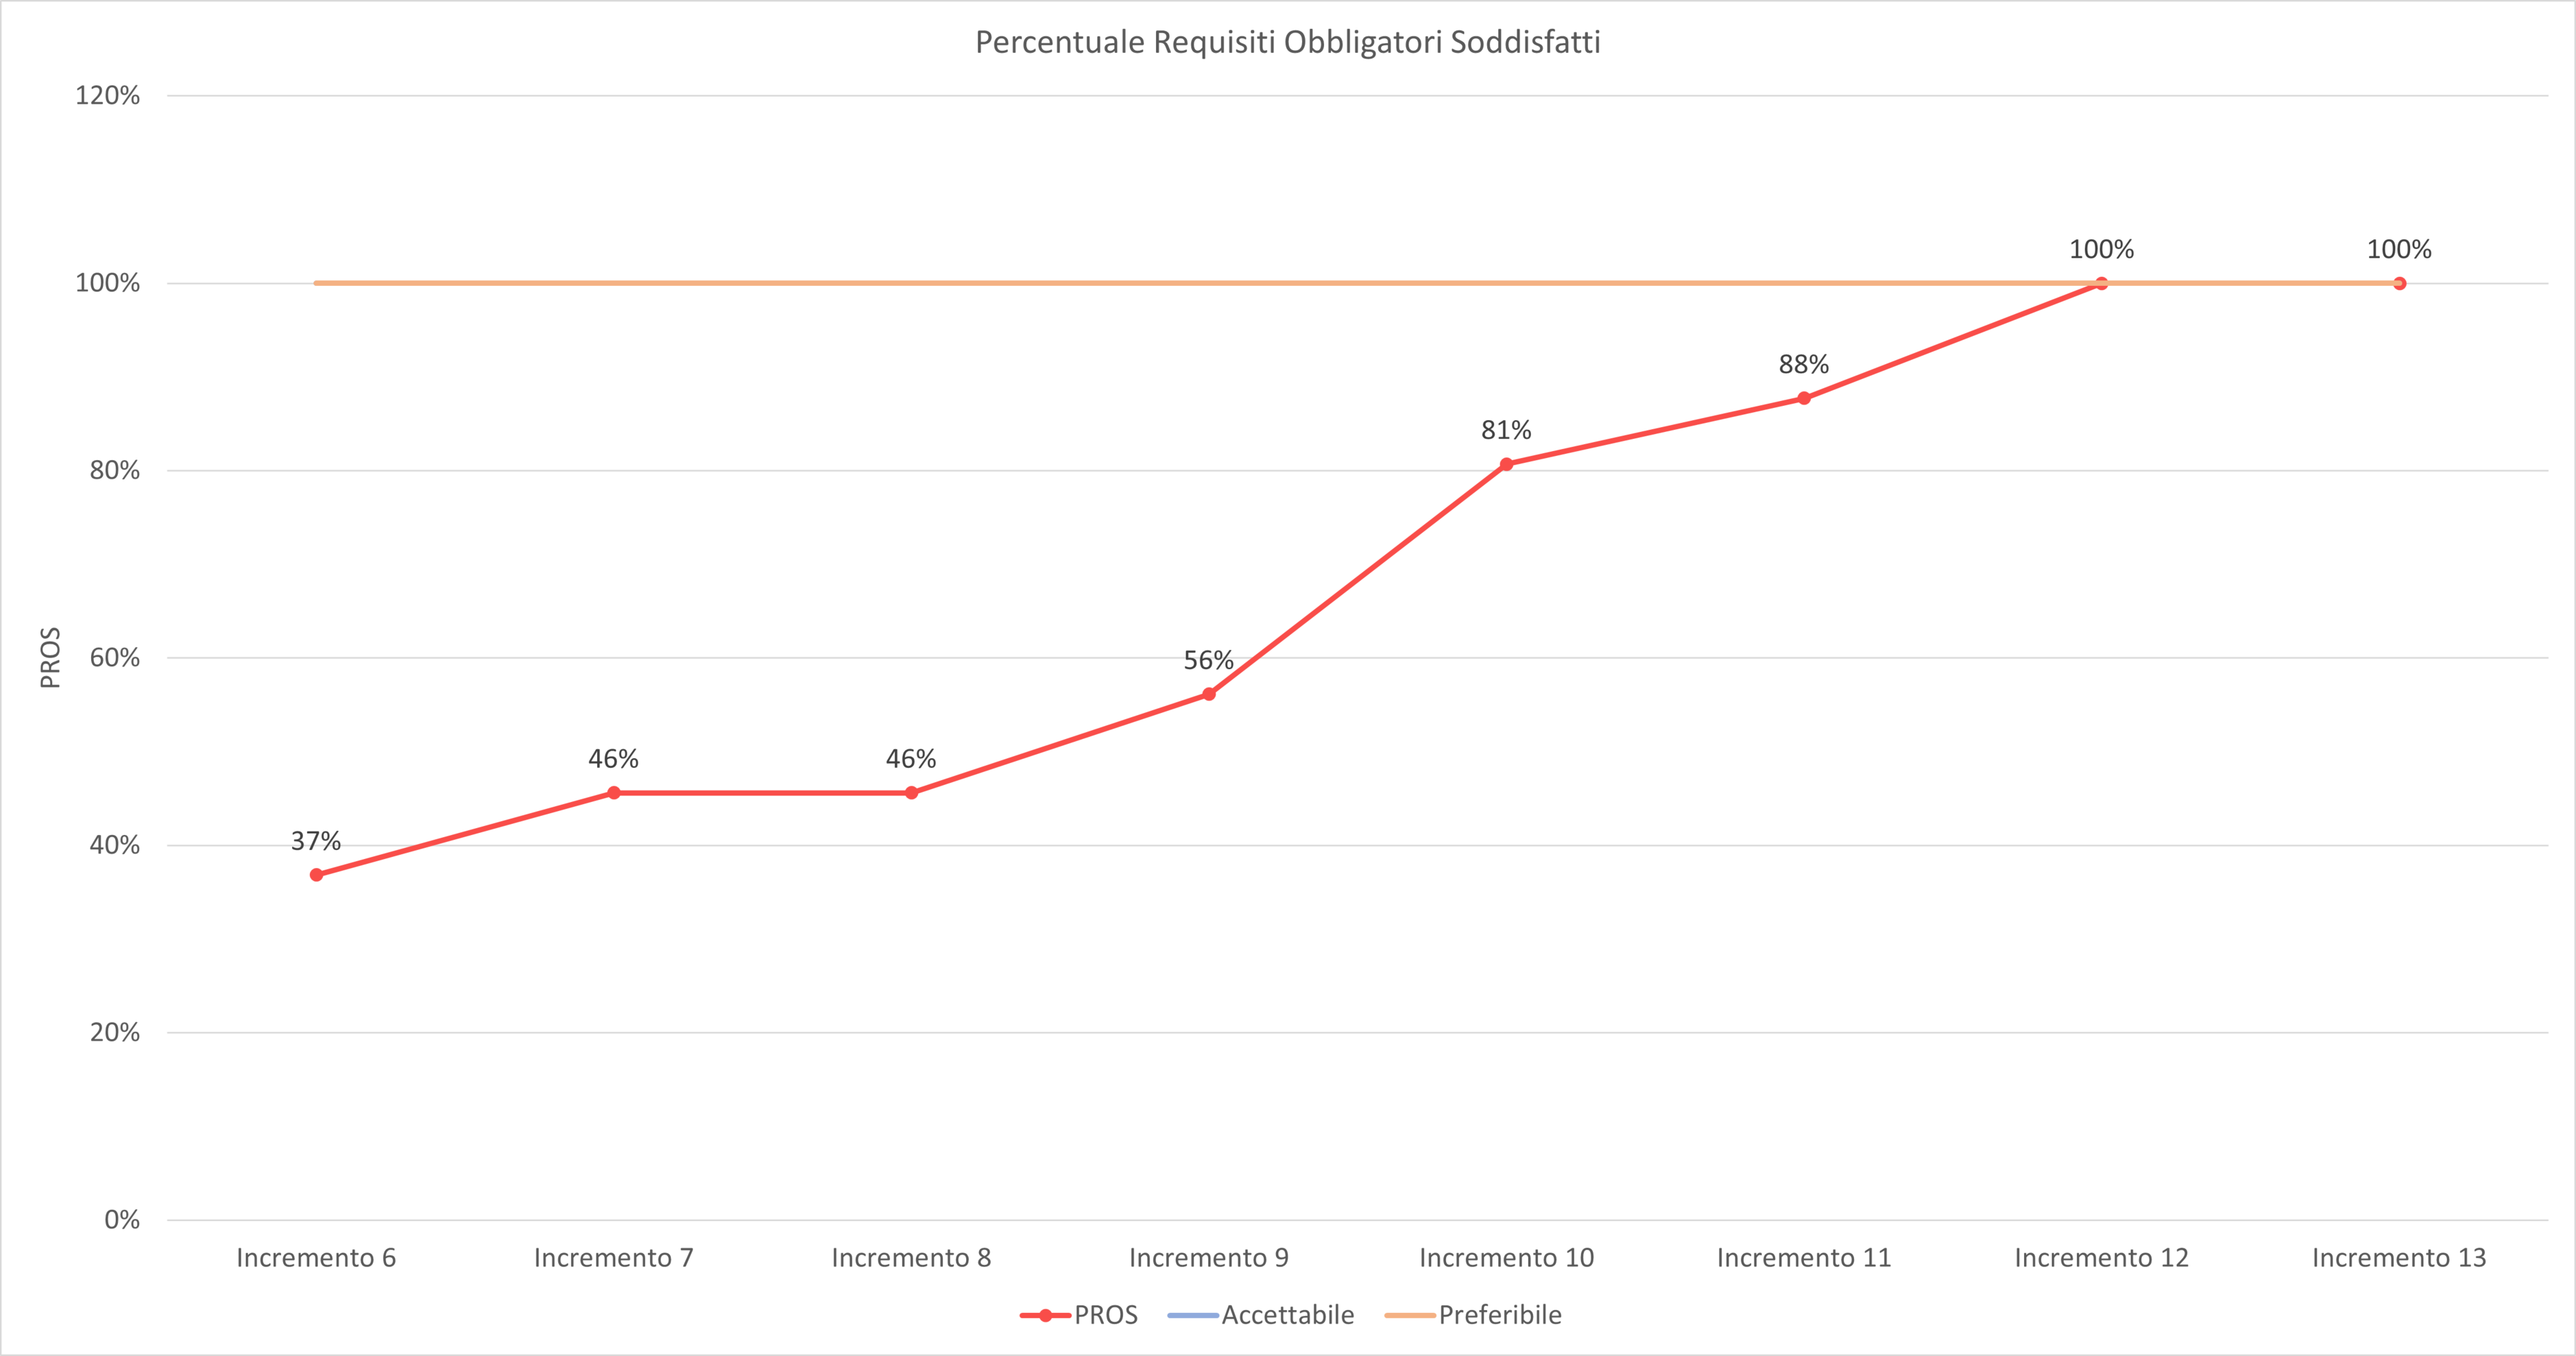
\includegraphics[scale=0.5]{sezioni/immagini/PROS.png}
    \centering
\end{figure}
\subsubsection{MPR02 - PRS (Percentuale Requisiti Soddisfatti)}
\begin{figure}[!ht]
    \caption{PRS (Percentuale Requisiti Soddisfatti)}
    \vspace{10px}
    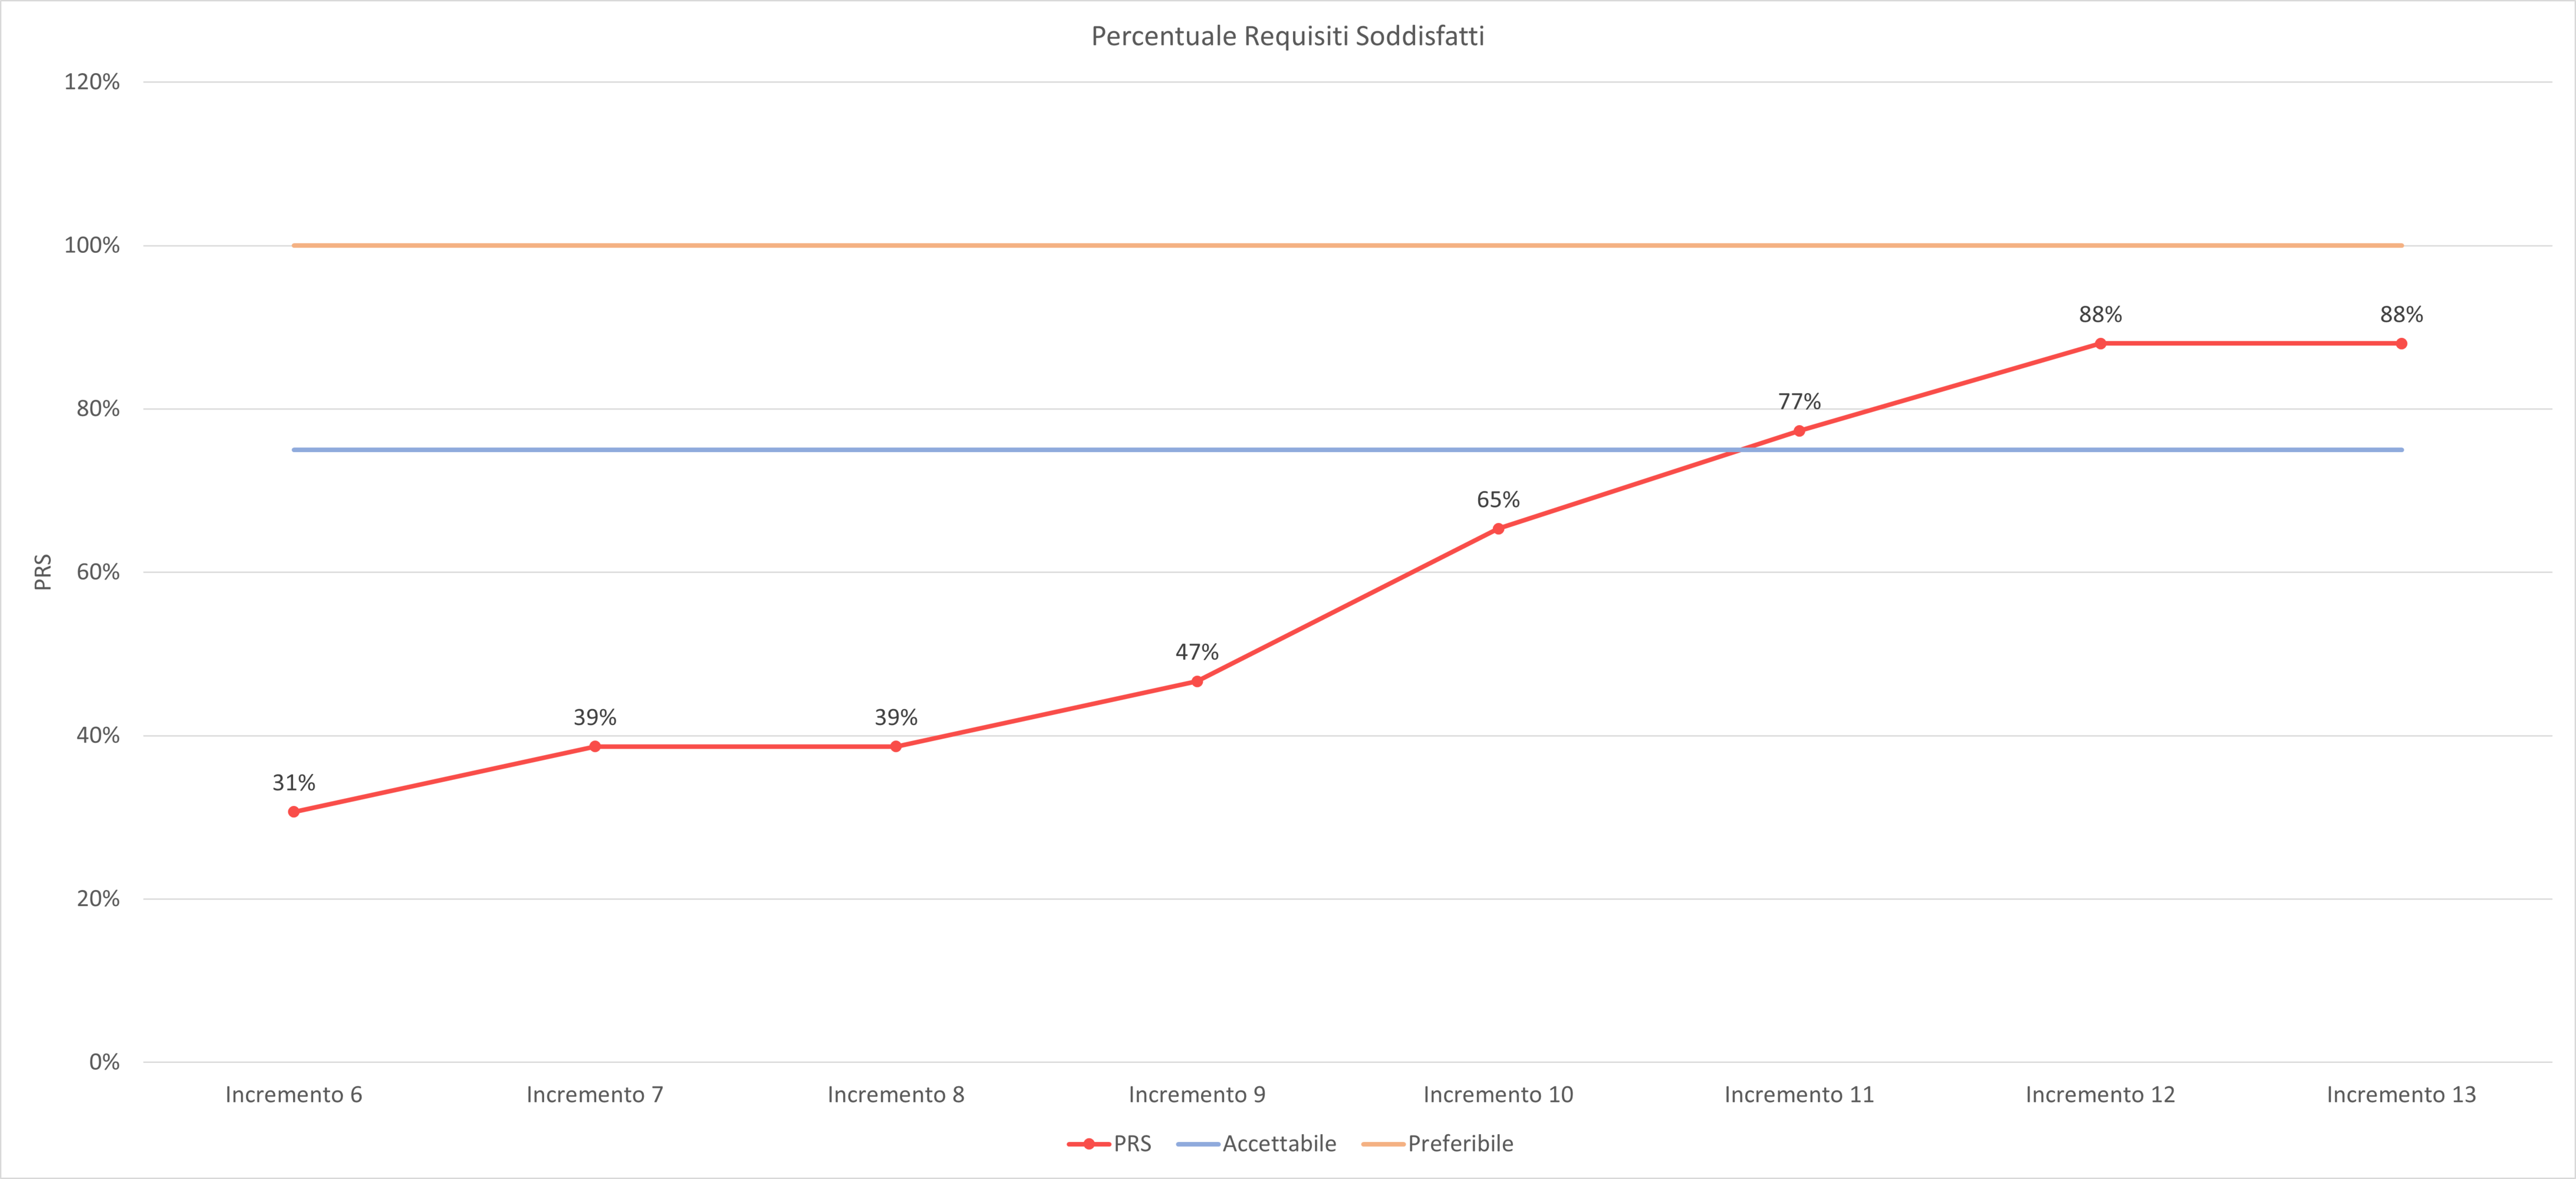
\includegraphics[scale=0.5]{sezioni/immagini/PRS.png}
    \centering
\end{figure}
\pagebreak
\subsubsection{MPR03 - Indice di Gulpease}
\subsubsubsection{Andamento complessivo}
\begin{center}
    \centering
    \rowcolors{2}{logo!10}{logo!40}
    \renewcommand{\arraystretch}{1.8}
    \label{tab:IndiciGulpease}
    \begin{longtable}[!h]{p{100px} p{50px} p{50px} p{50px} p{50px} p{50px} p{50px}}
        \caption{Esiti verifica con Gulpease}                                                                                        \\
        \rowcolor{logo!70}   \textbf{Documento} & \textbf{A} & \textbf{C} & \textbf{PA} & \textbf{PD} & \textbf{VC} & \textbf{Esito} \\
        \textit{Norme di Progetto}              & 68         & 68         & 72          & 68          &             & Superato       \\
        \textit{Piano di Progetto}              & 73         & 73         & 69          & 73          &             & Superato       \\
        \textit{Analisi dei Requisiti}          & 71         & 71         & 68          & 67          &             & Superato       \\
        \textit{Piano di Qualifica}             & 69         & 69         & 69          & 69          &             & Superato       \\
        \textit{Studio di Fattibilità}          & 74         & 74         & /           & /           &             & Superato       \\
        \textit{Maintainer Manual}              & /          & /          & /           & 70          &             & Superato       \\
        \textit{User Manual}                    & /          & /          & /           & 78          &             & Superato       \\
        \textit{Glossario}                      & 49         & 49         & 49          & 49          &             & Superato       \\
        \textit{Verbali interni (media)}        & 67         & 67         & 56          & 59          &             & Superato       \\
        \textit{Verbali esterni (media)}        & 71         & 71         & 60          & 57          &             & Superato       \\
        \rowcolor{white}
    \end{longtable}
\end{center}
\begin{figure}[!ht]
    \caption{Indice di Gulpease: \textit{Andamento complessivo}}
    \vspace{10px}
    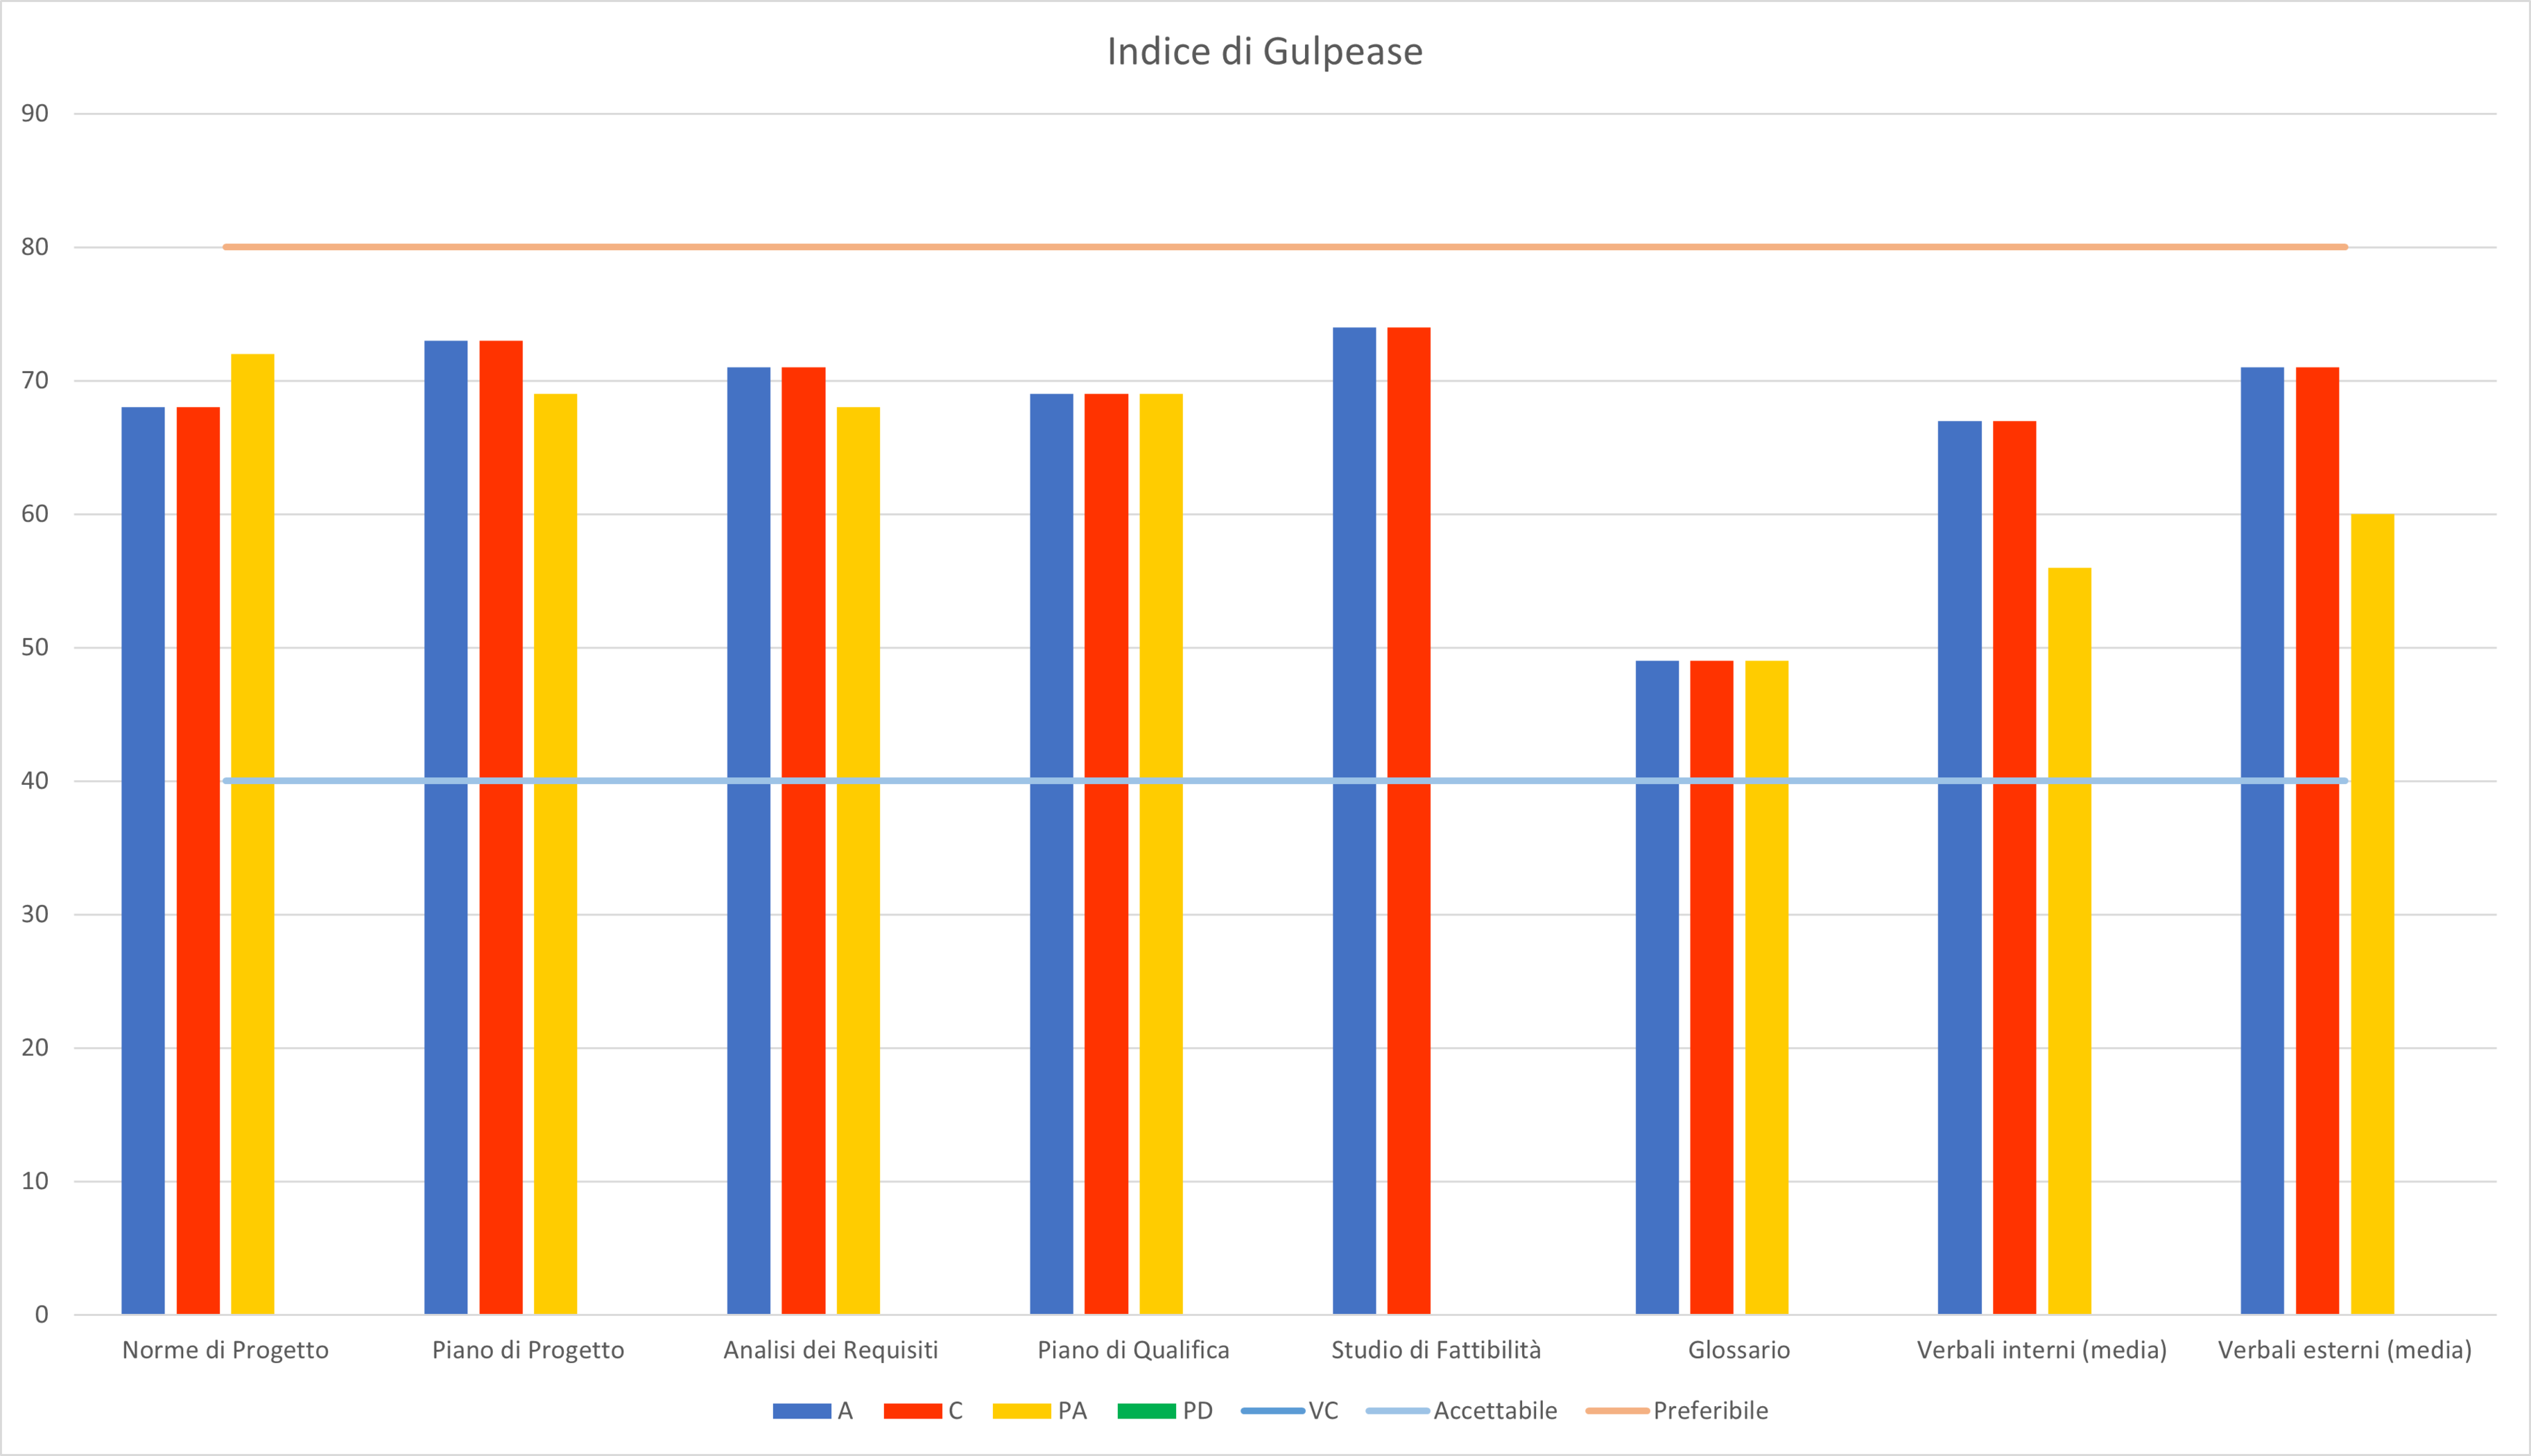
\includegraphics[scale=0.5]{sezioni/immagini/GulpeaseGenerale.png}
    \centering
\end{figure}
\pagebreak
\subsubsubsection{Andamento per documento}
\begin{figure}[!ht]
    \caption{Indice di Gulpease: \textit{Norme di Progetto}}
    \vspace{10px}
    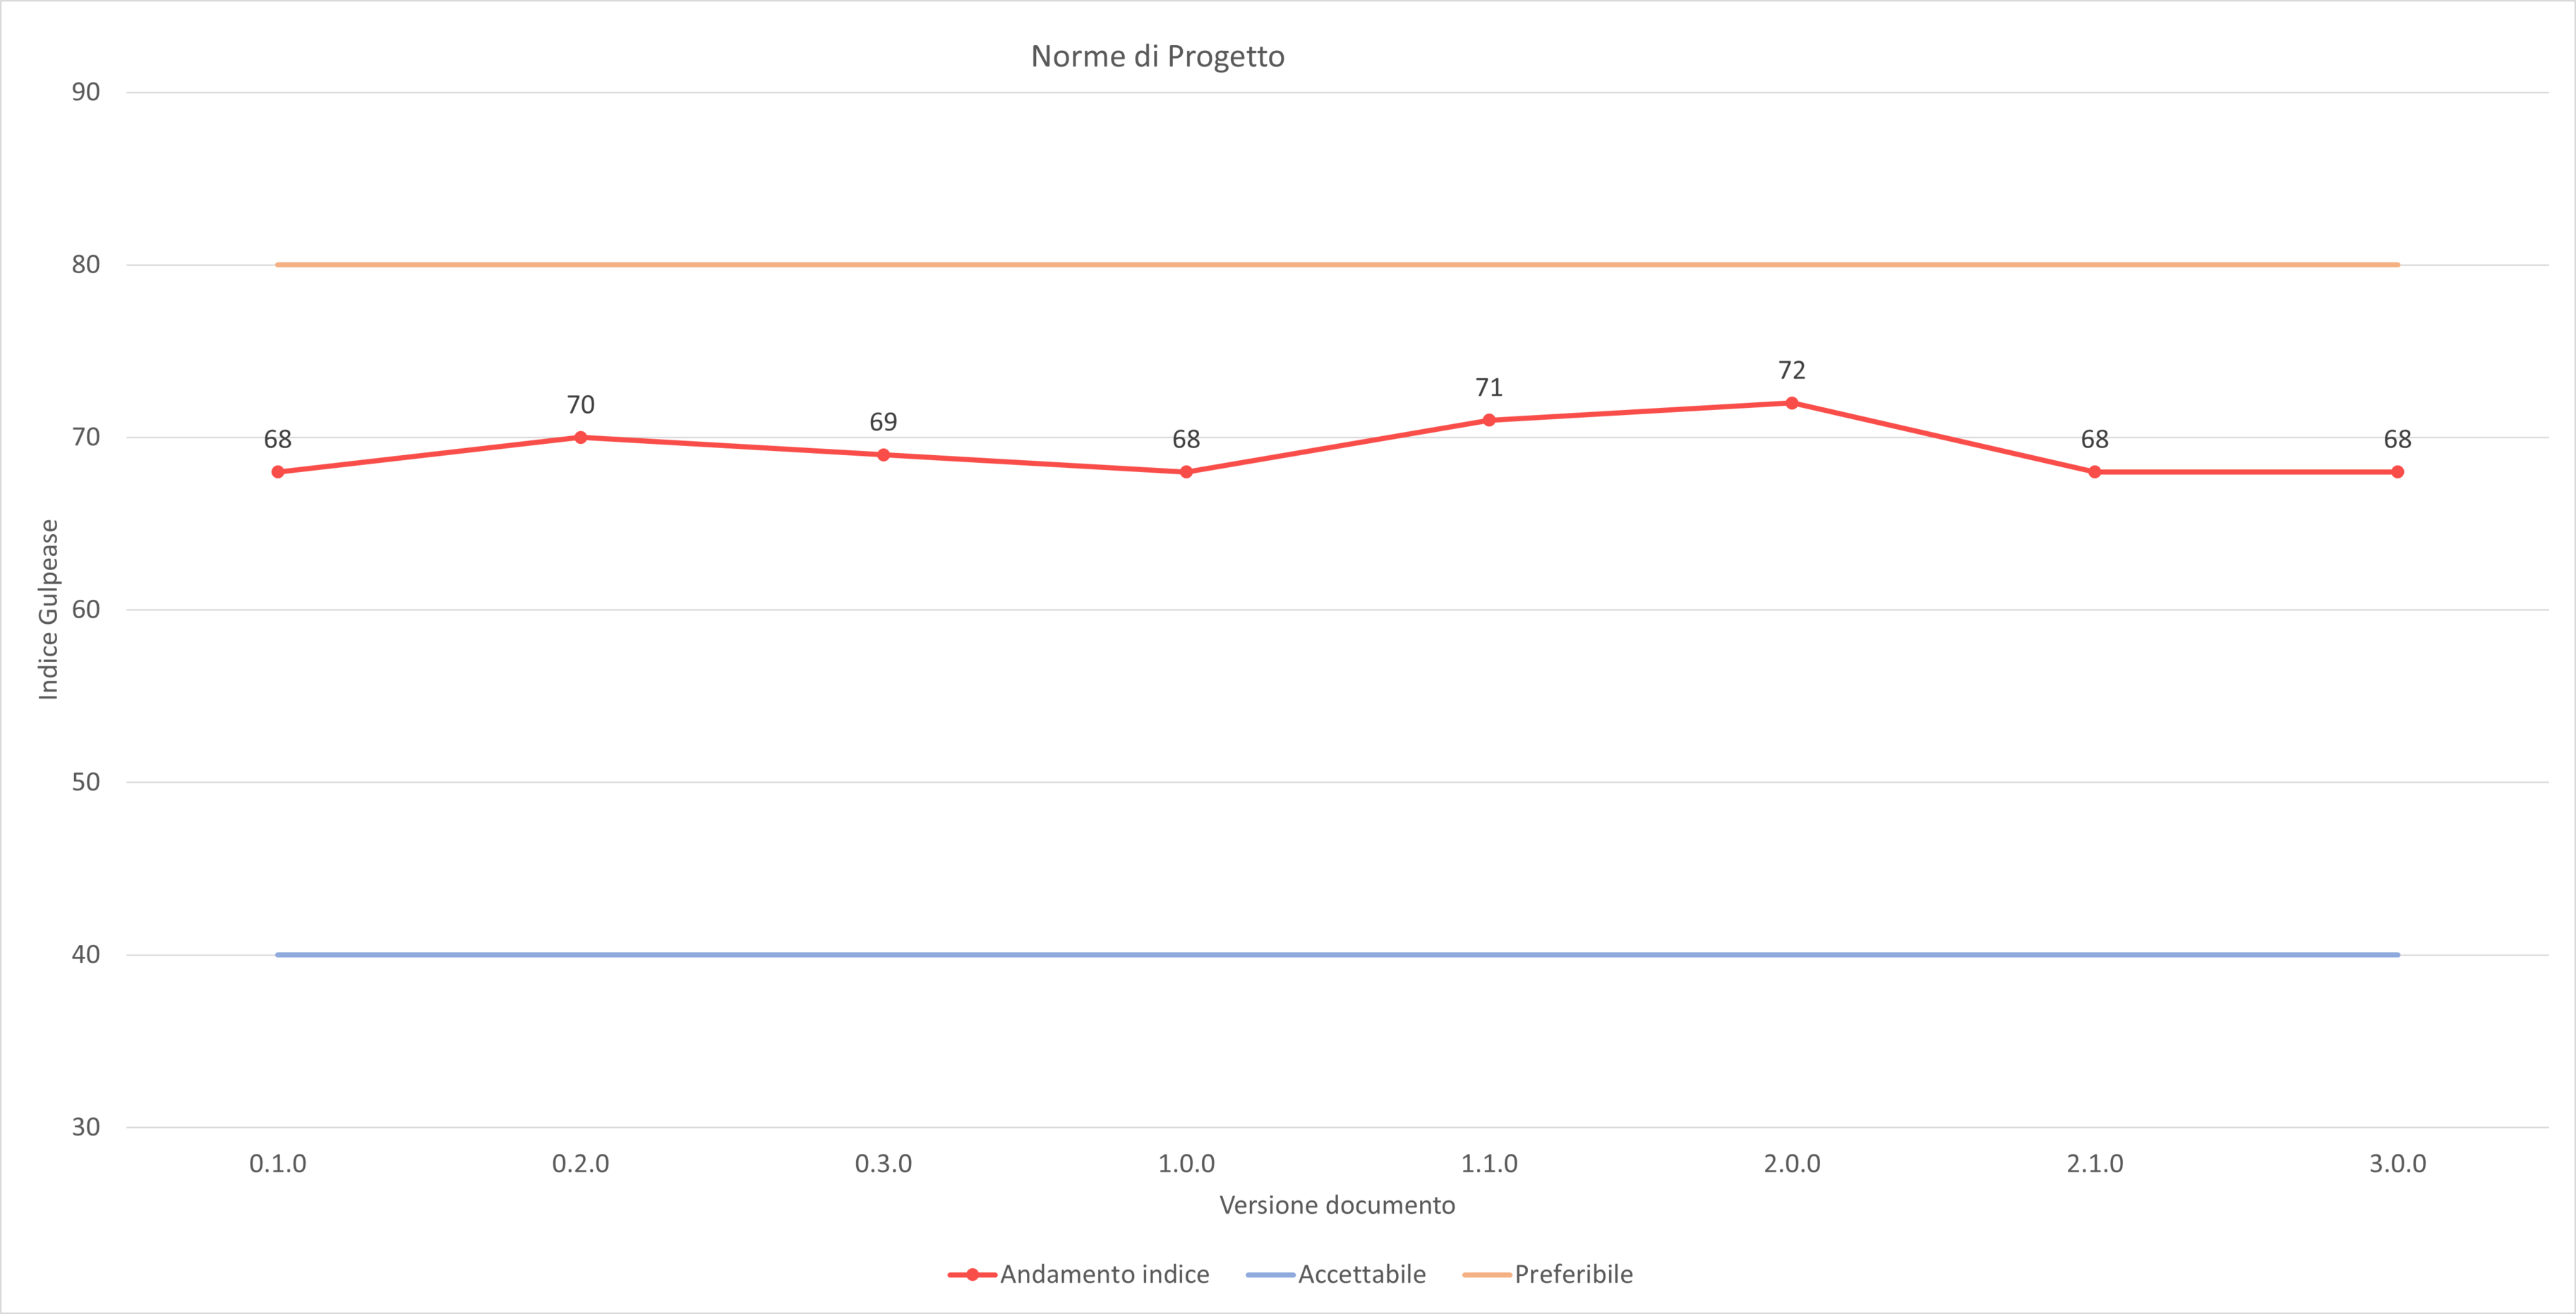
\includegraphics[scale=0.5]{sezioni/immagini/NormeGulpease.png}
    \centering
\end{figure}
\begin{figure}[!ht]
    \caption{Indice di Gulpease: \textit{Piano di Progetto}}
    \vspace{10px}
    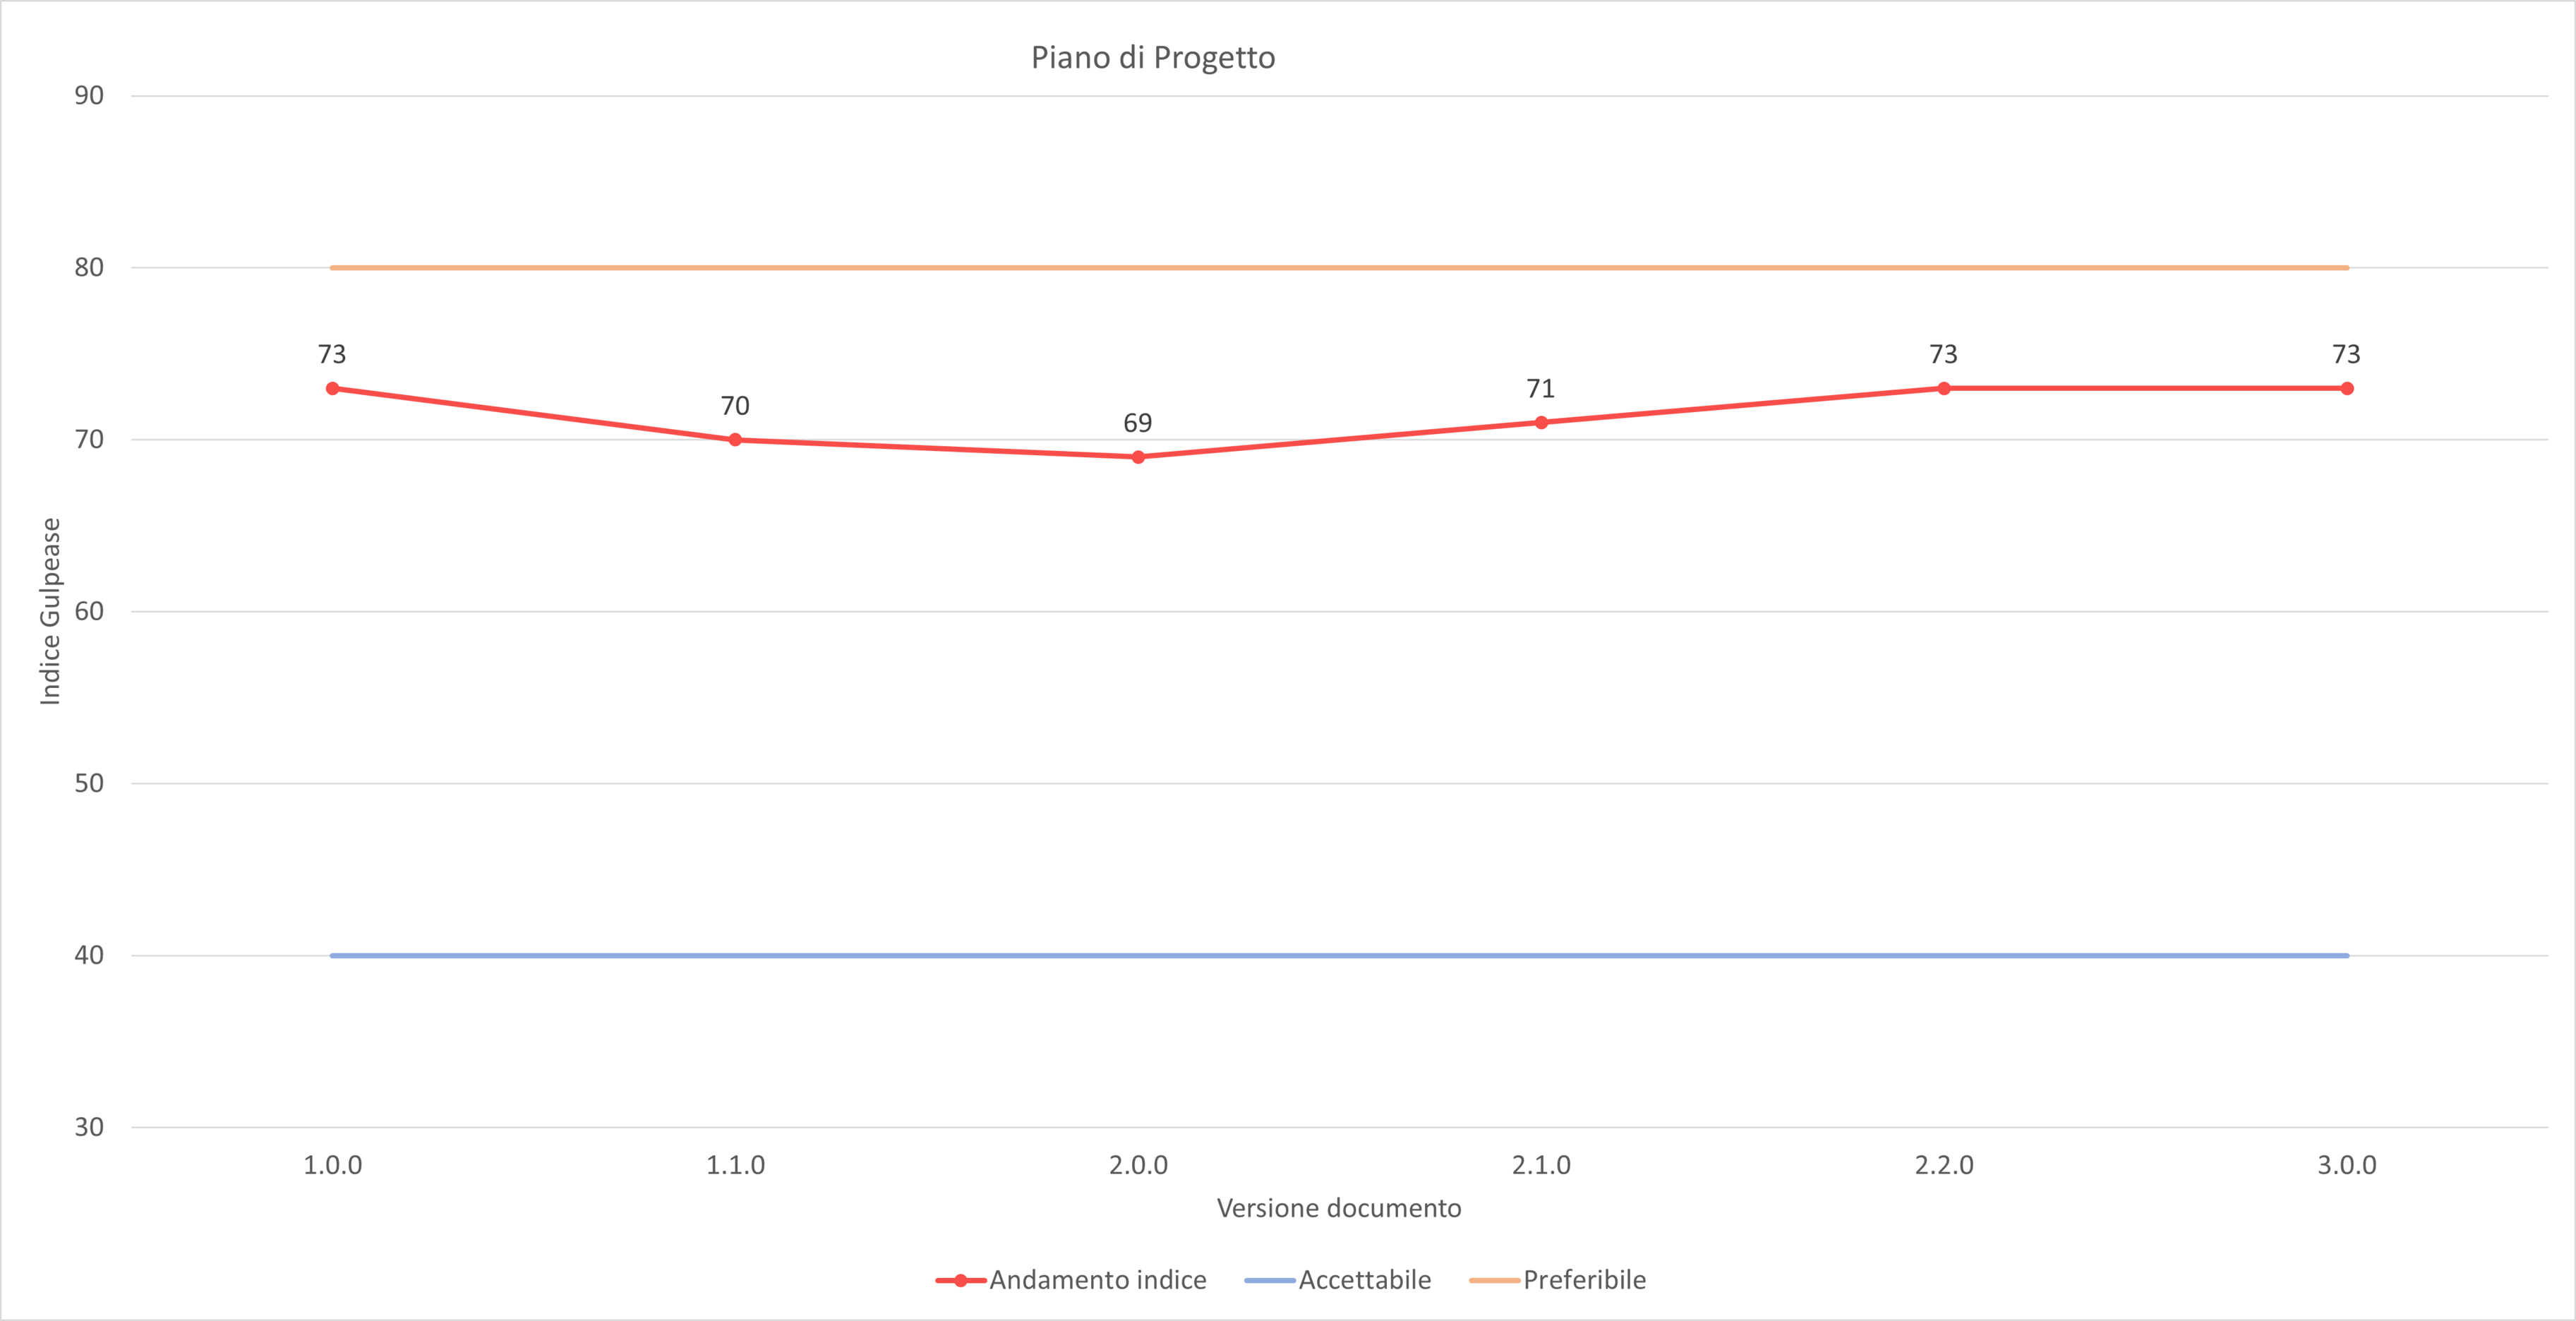
\includegraphics[scale=0.5]{sezioni/immagini/PianoProgettoGulpease.png}
    \centering
\end{figure}
\pagebreak
\begin{figure}[!ht]
    \caption{Indice di Gulpease: \textit{Analisi dei Requisiti}}
    \vspace{10px}
    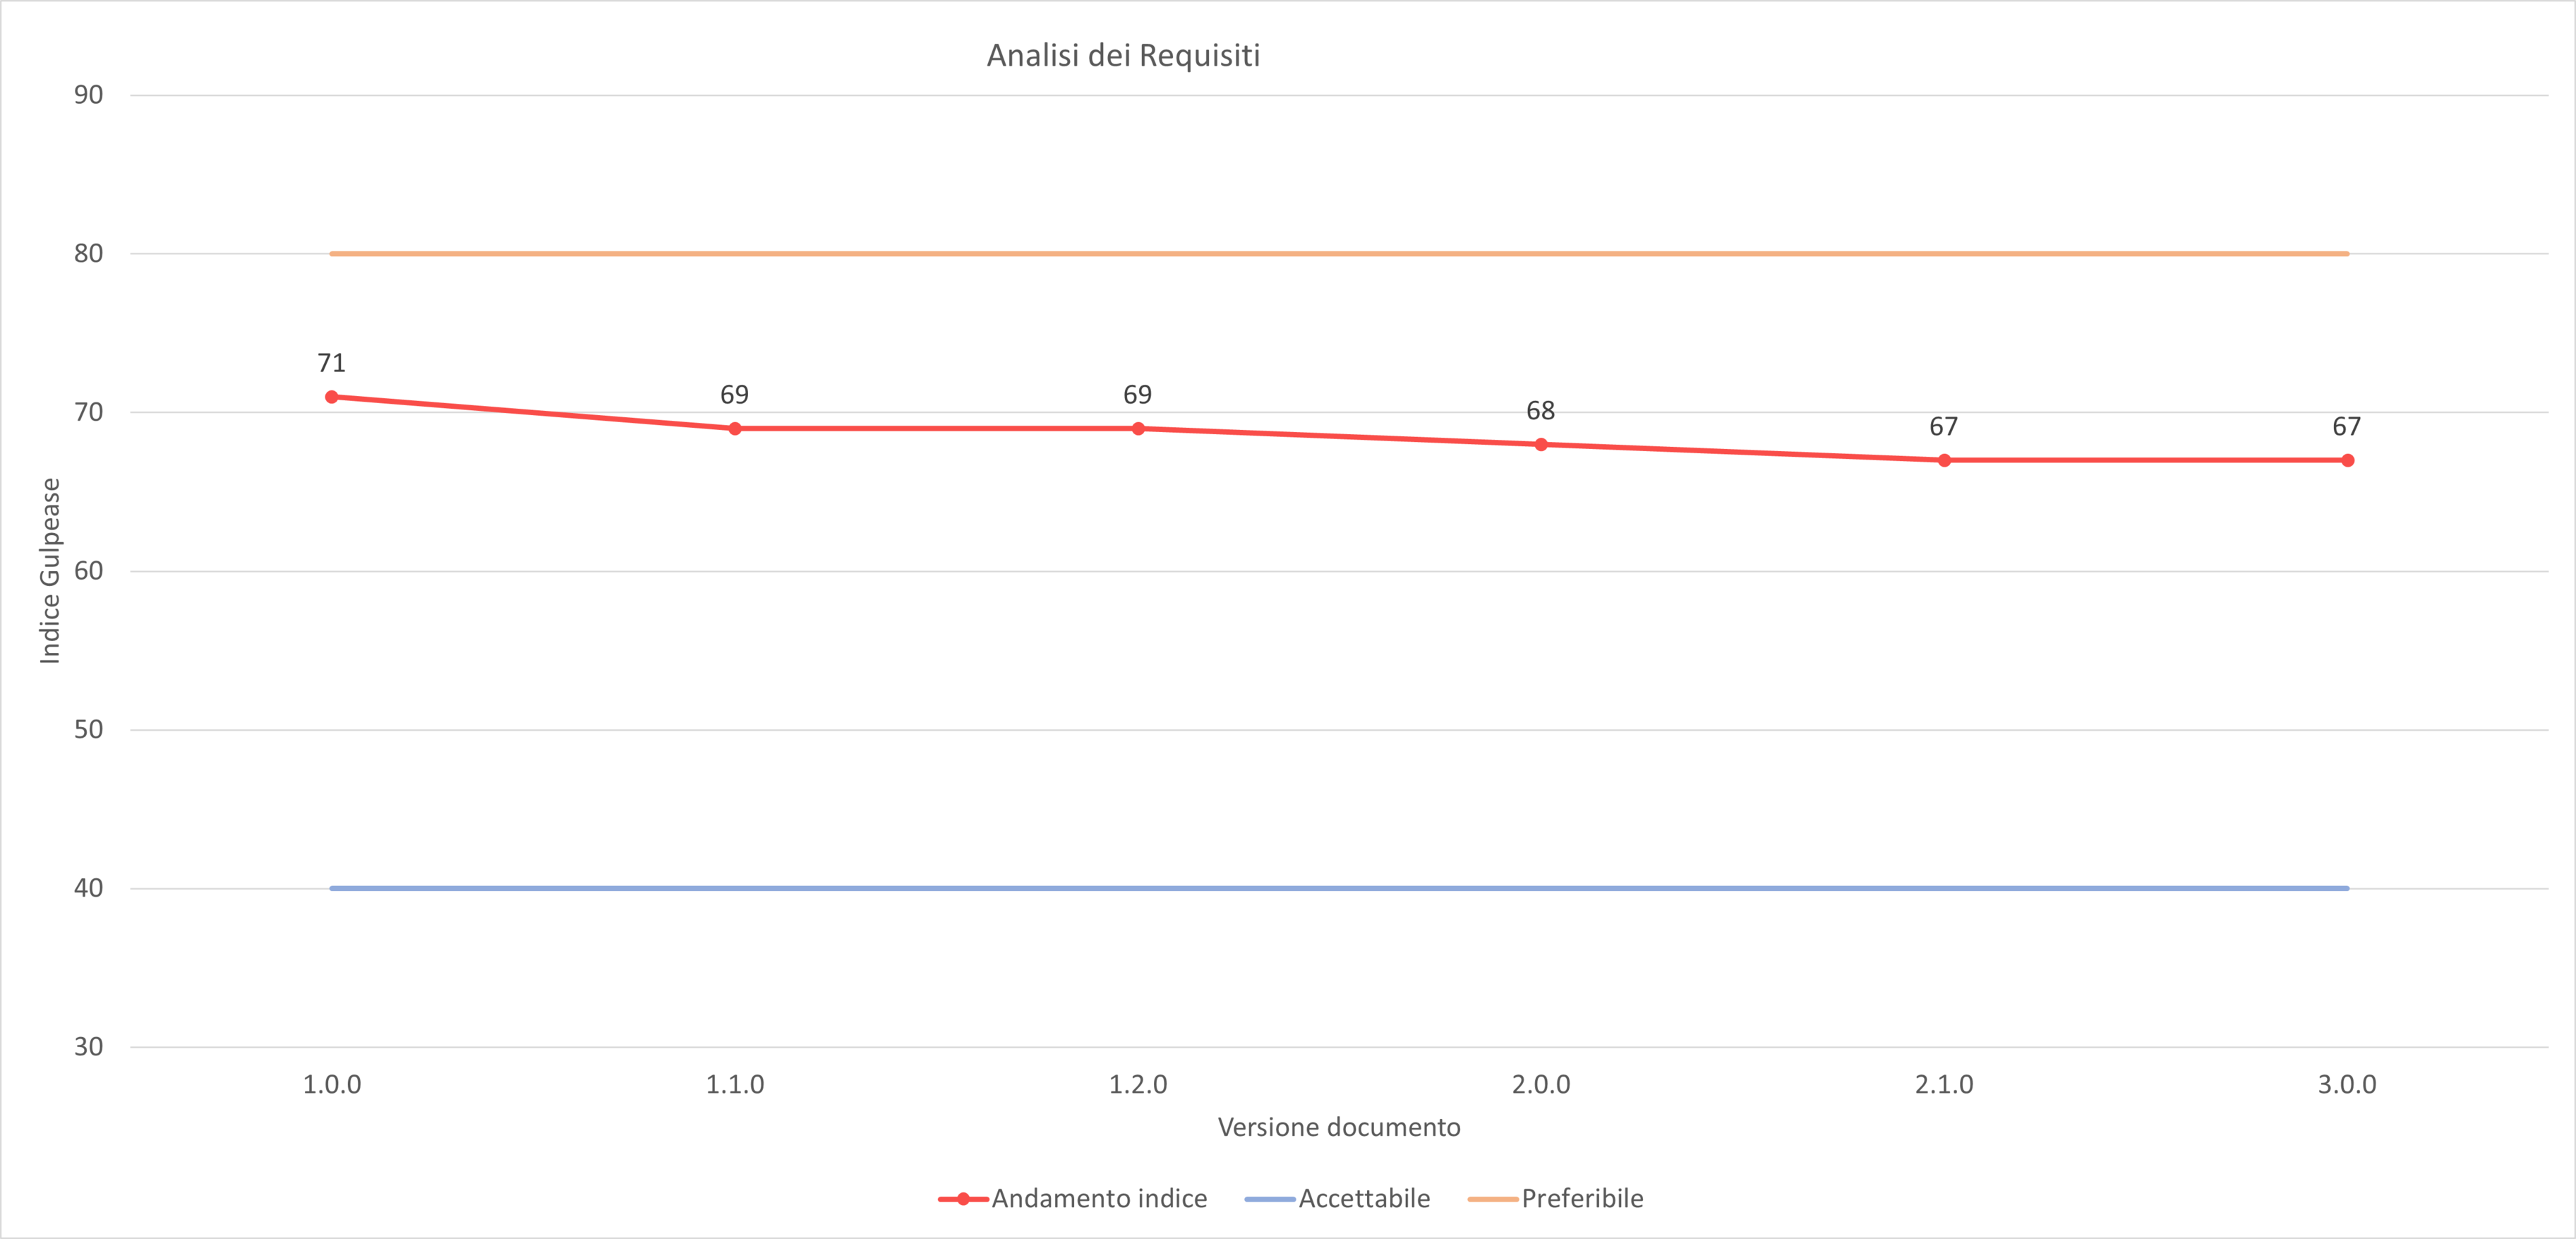
\includegraphics[scale=0.5]{sezioni/immagini/AnalisiGulpease.png}
    \centering
\end{figure}
\begin{figure}[!ht]
    \caption{Indice di Gulpease: \textit{Piano di Qualifica}}
    \vspace{10px}
    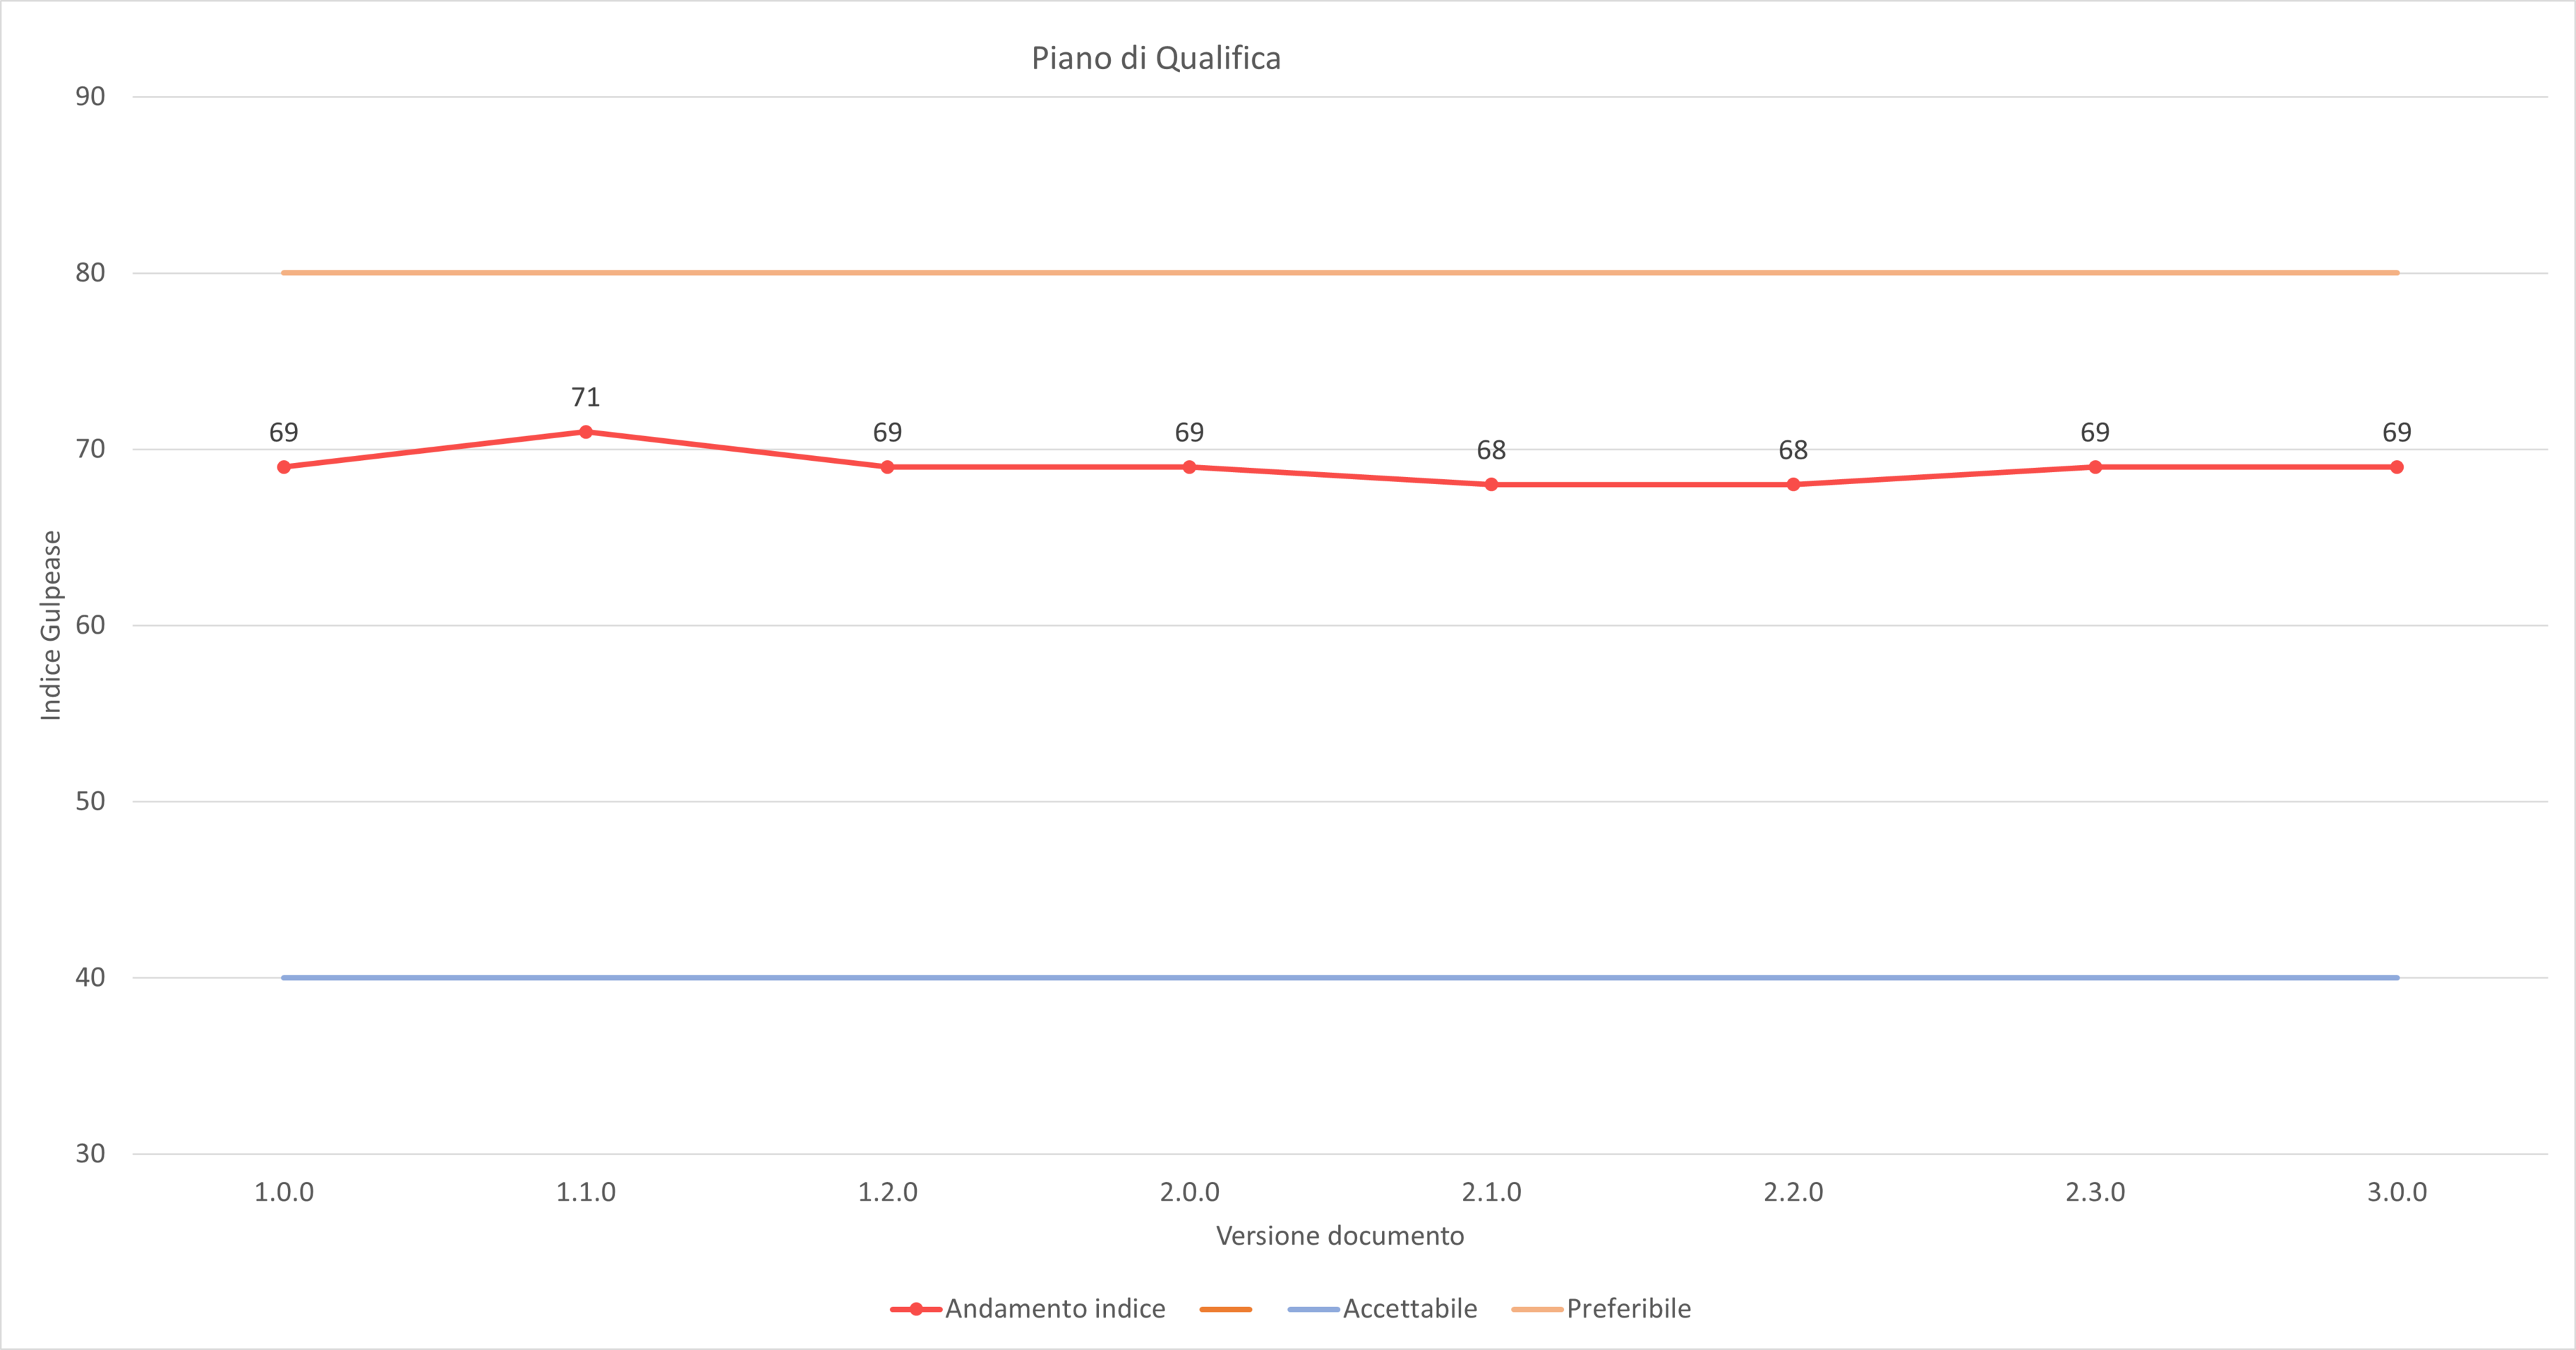
\includegraphics[scale=0.5]{sezioni/immagini/PianoQualificaGulpease.png}
    \centering
\end{figure}
\pagebreak
\begin{figure}[!ht]
    \caption{Indice di Gulpease: \textit{Studio di Fattibilità}}
    \vspace{10px}
    \includegraphics[scale=0.5]{sezioni/immagini/FattibilitàGulpease.png}
    \centering
\end{figure}
\begin{figure}[!ht]
    \caption{Indice di Gulpease: \textit{Glossario}}
    \vspace{10px}
    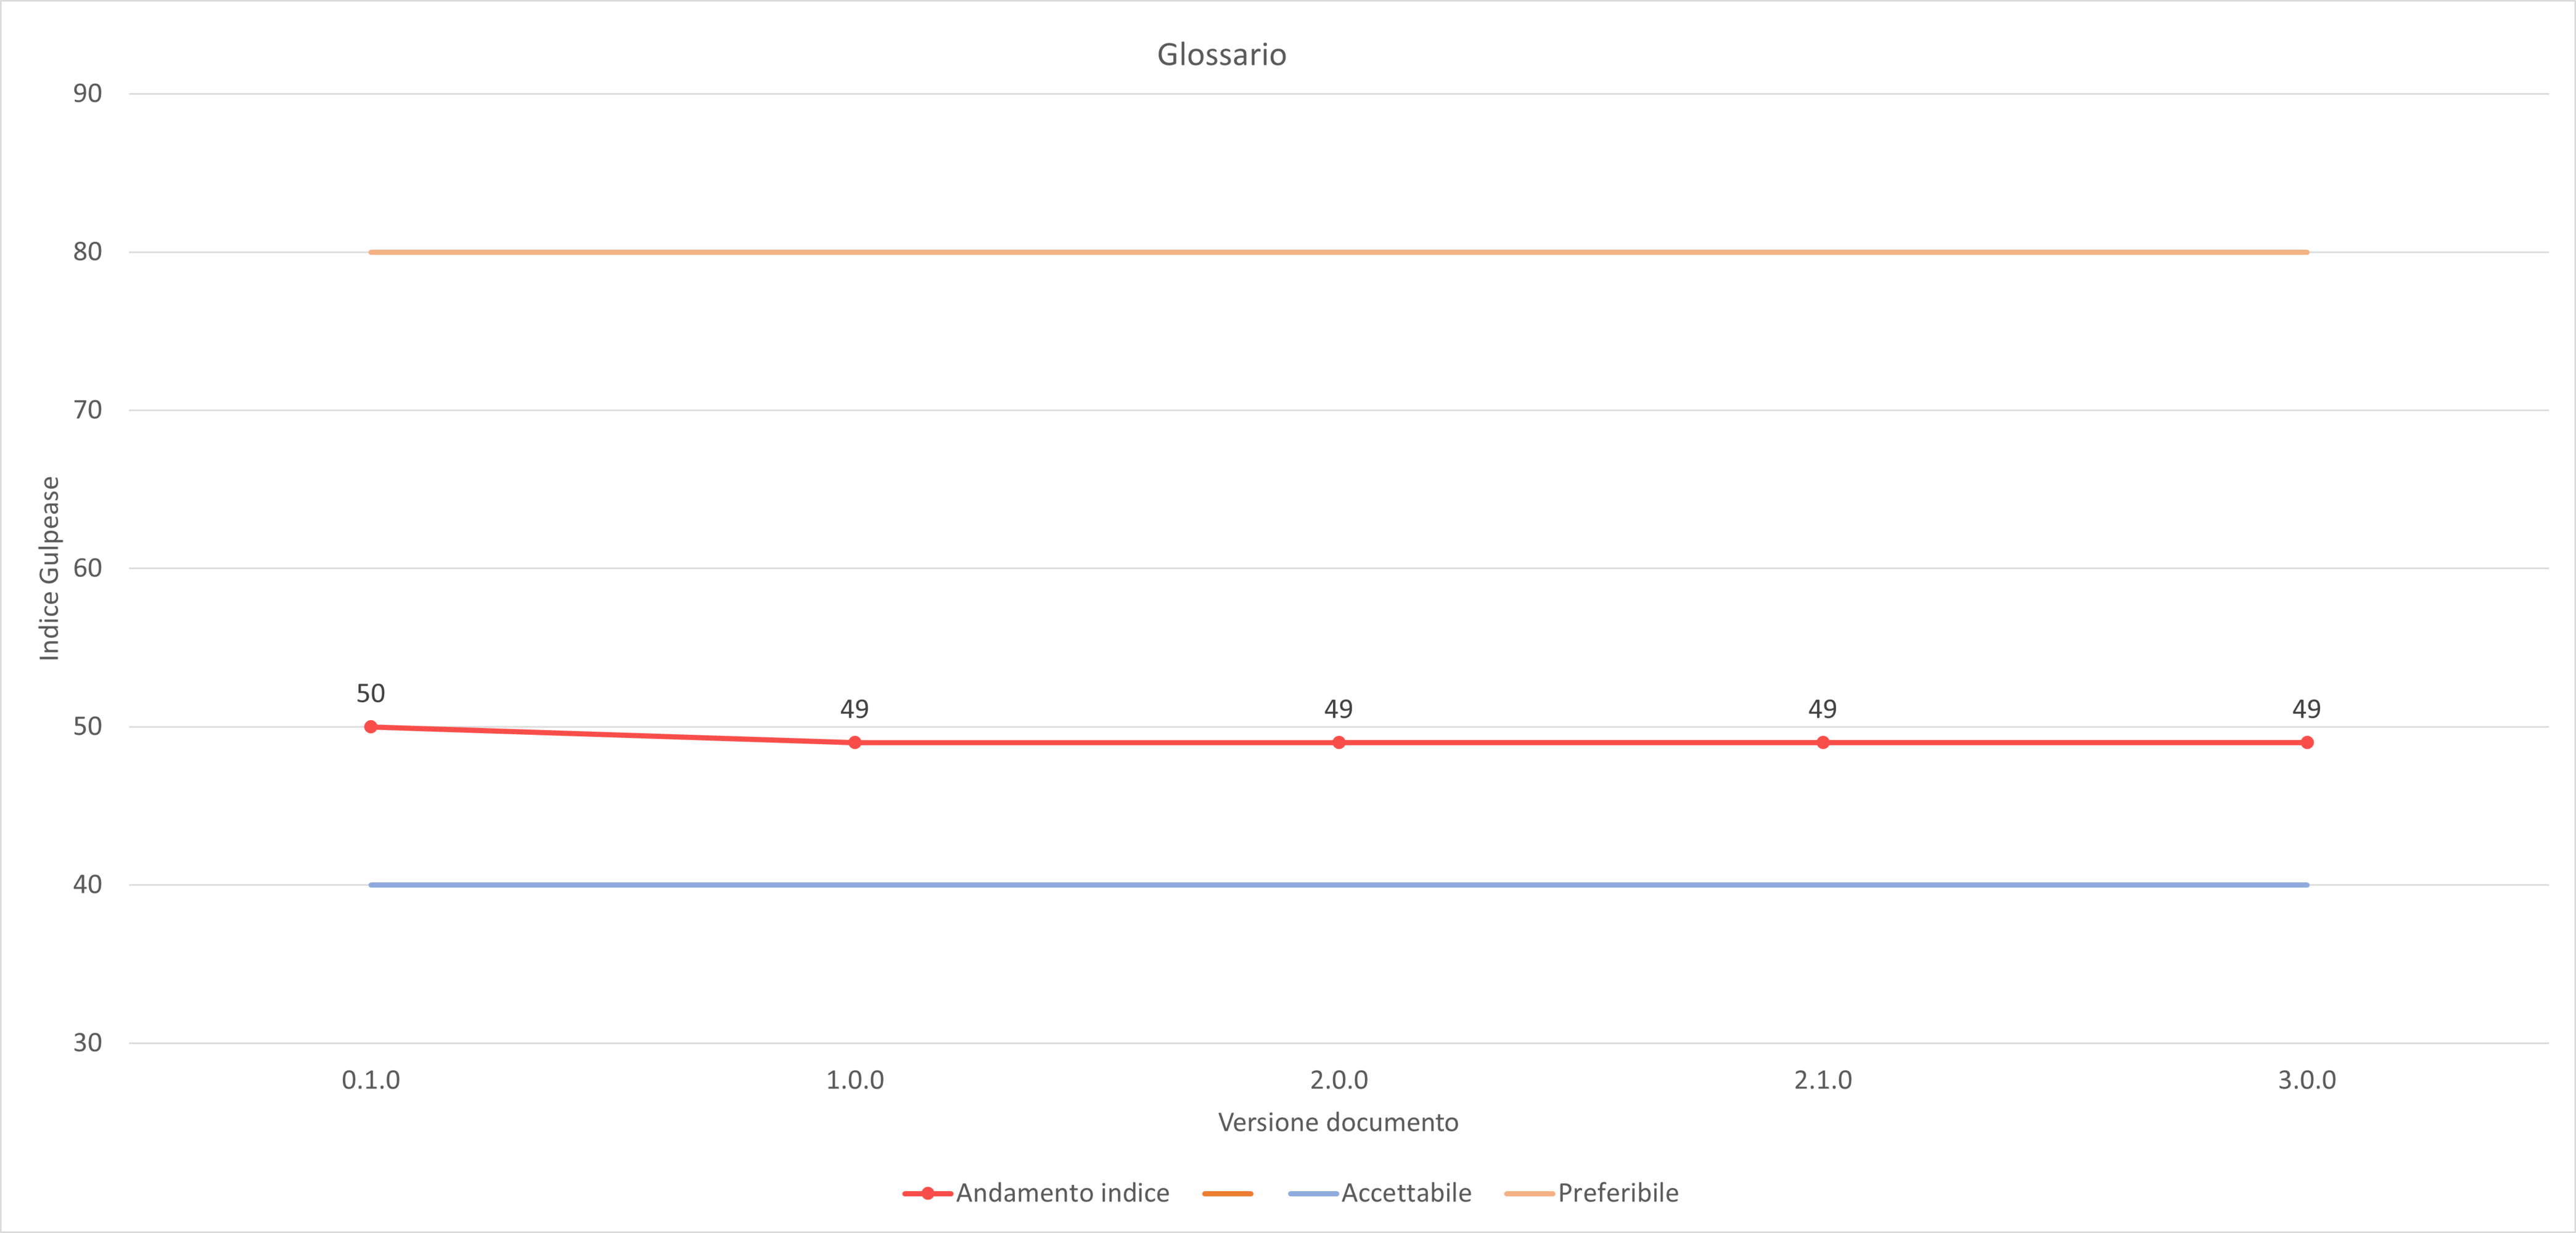
\includegraphics[scale=0.5]{sezioni/immagini/GlossarioGulpease.png}
    \centering
\end{figure}
\pagebreak
\begin{figure}[!ht]
    \caption{Indice di Gulpease: \textit{Maintainer Manual}}
    \vspace{10px}
    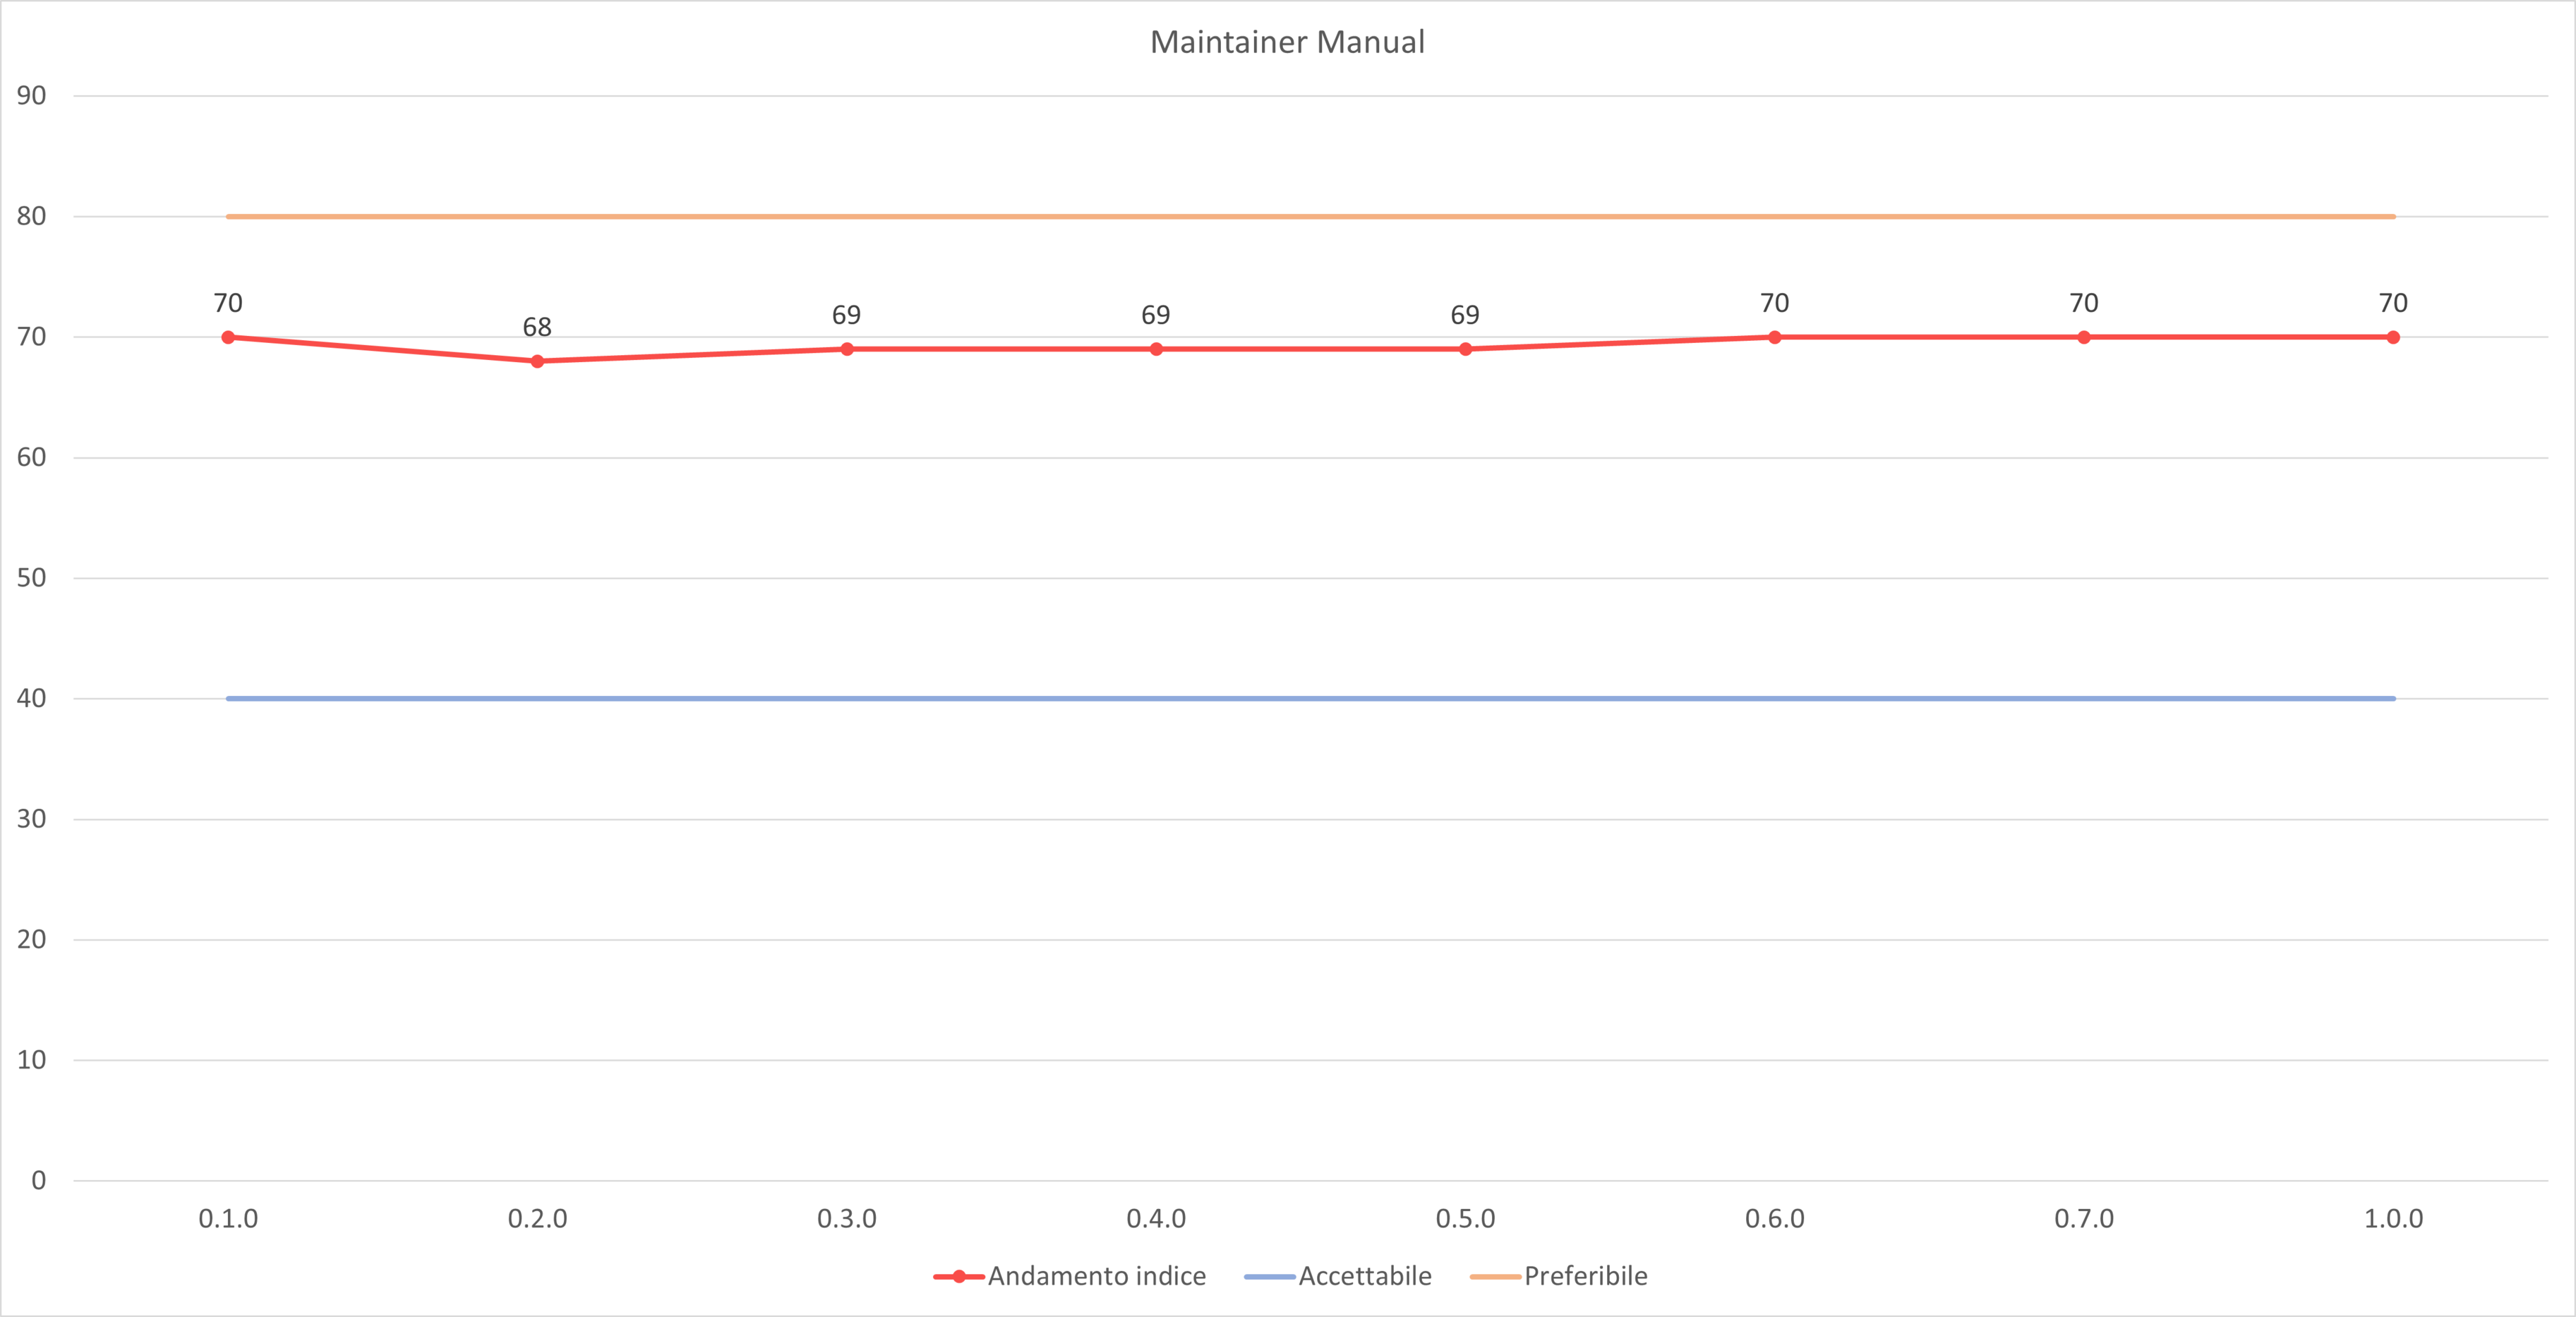
\includegraphics[scale=0.5]{sezioni/immagini/MaintainerManualGulpease.png}
    \centering
\end{figure}
\begin{figure}[!ht]
    \caption{Indice di Gulpease: \textit{User Manual}}
    \vspace{10px}
    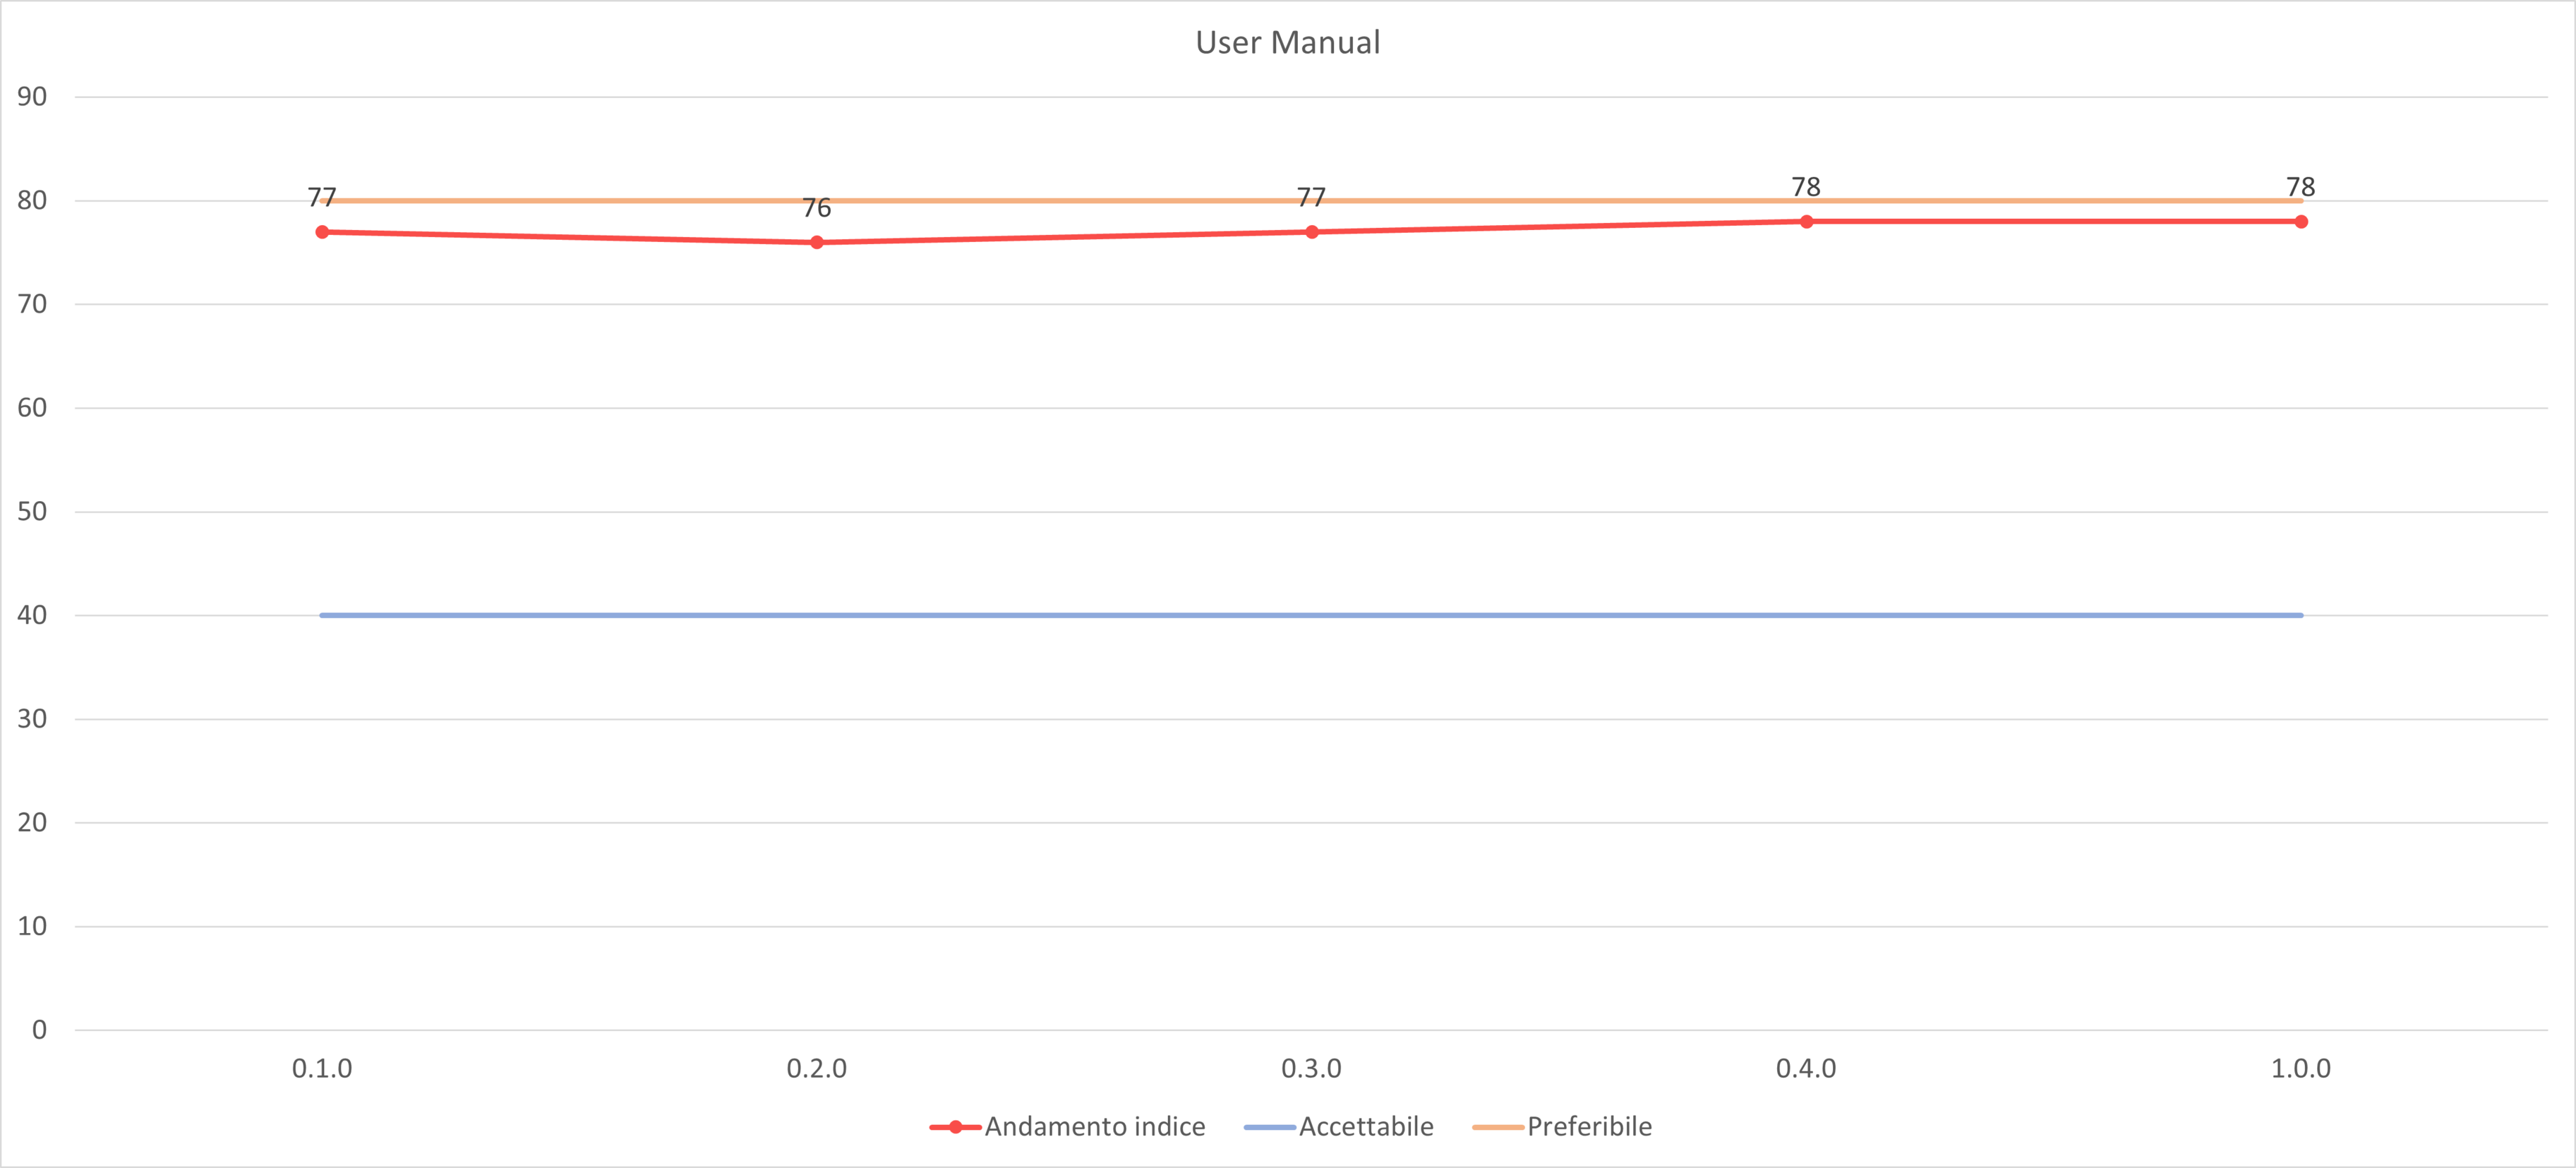
\includegraphics[scale=0.5]{sezioni/immagini/UserManualGulpease.png}
    \centering
\end{figure}
\pagebreak
\subsubsection{MPR04 - Correttezza ortografica}
\begin{figure}[!ht]
    \caption{Correttezza ortografica}
    \vspace{10px}
    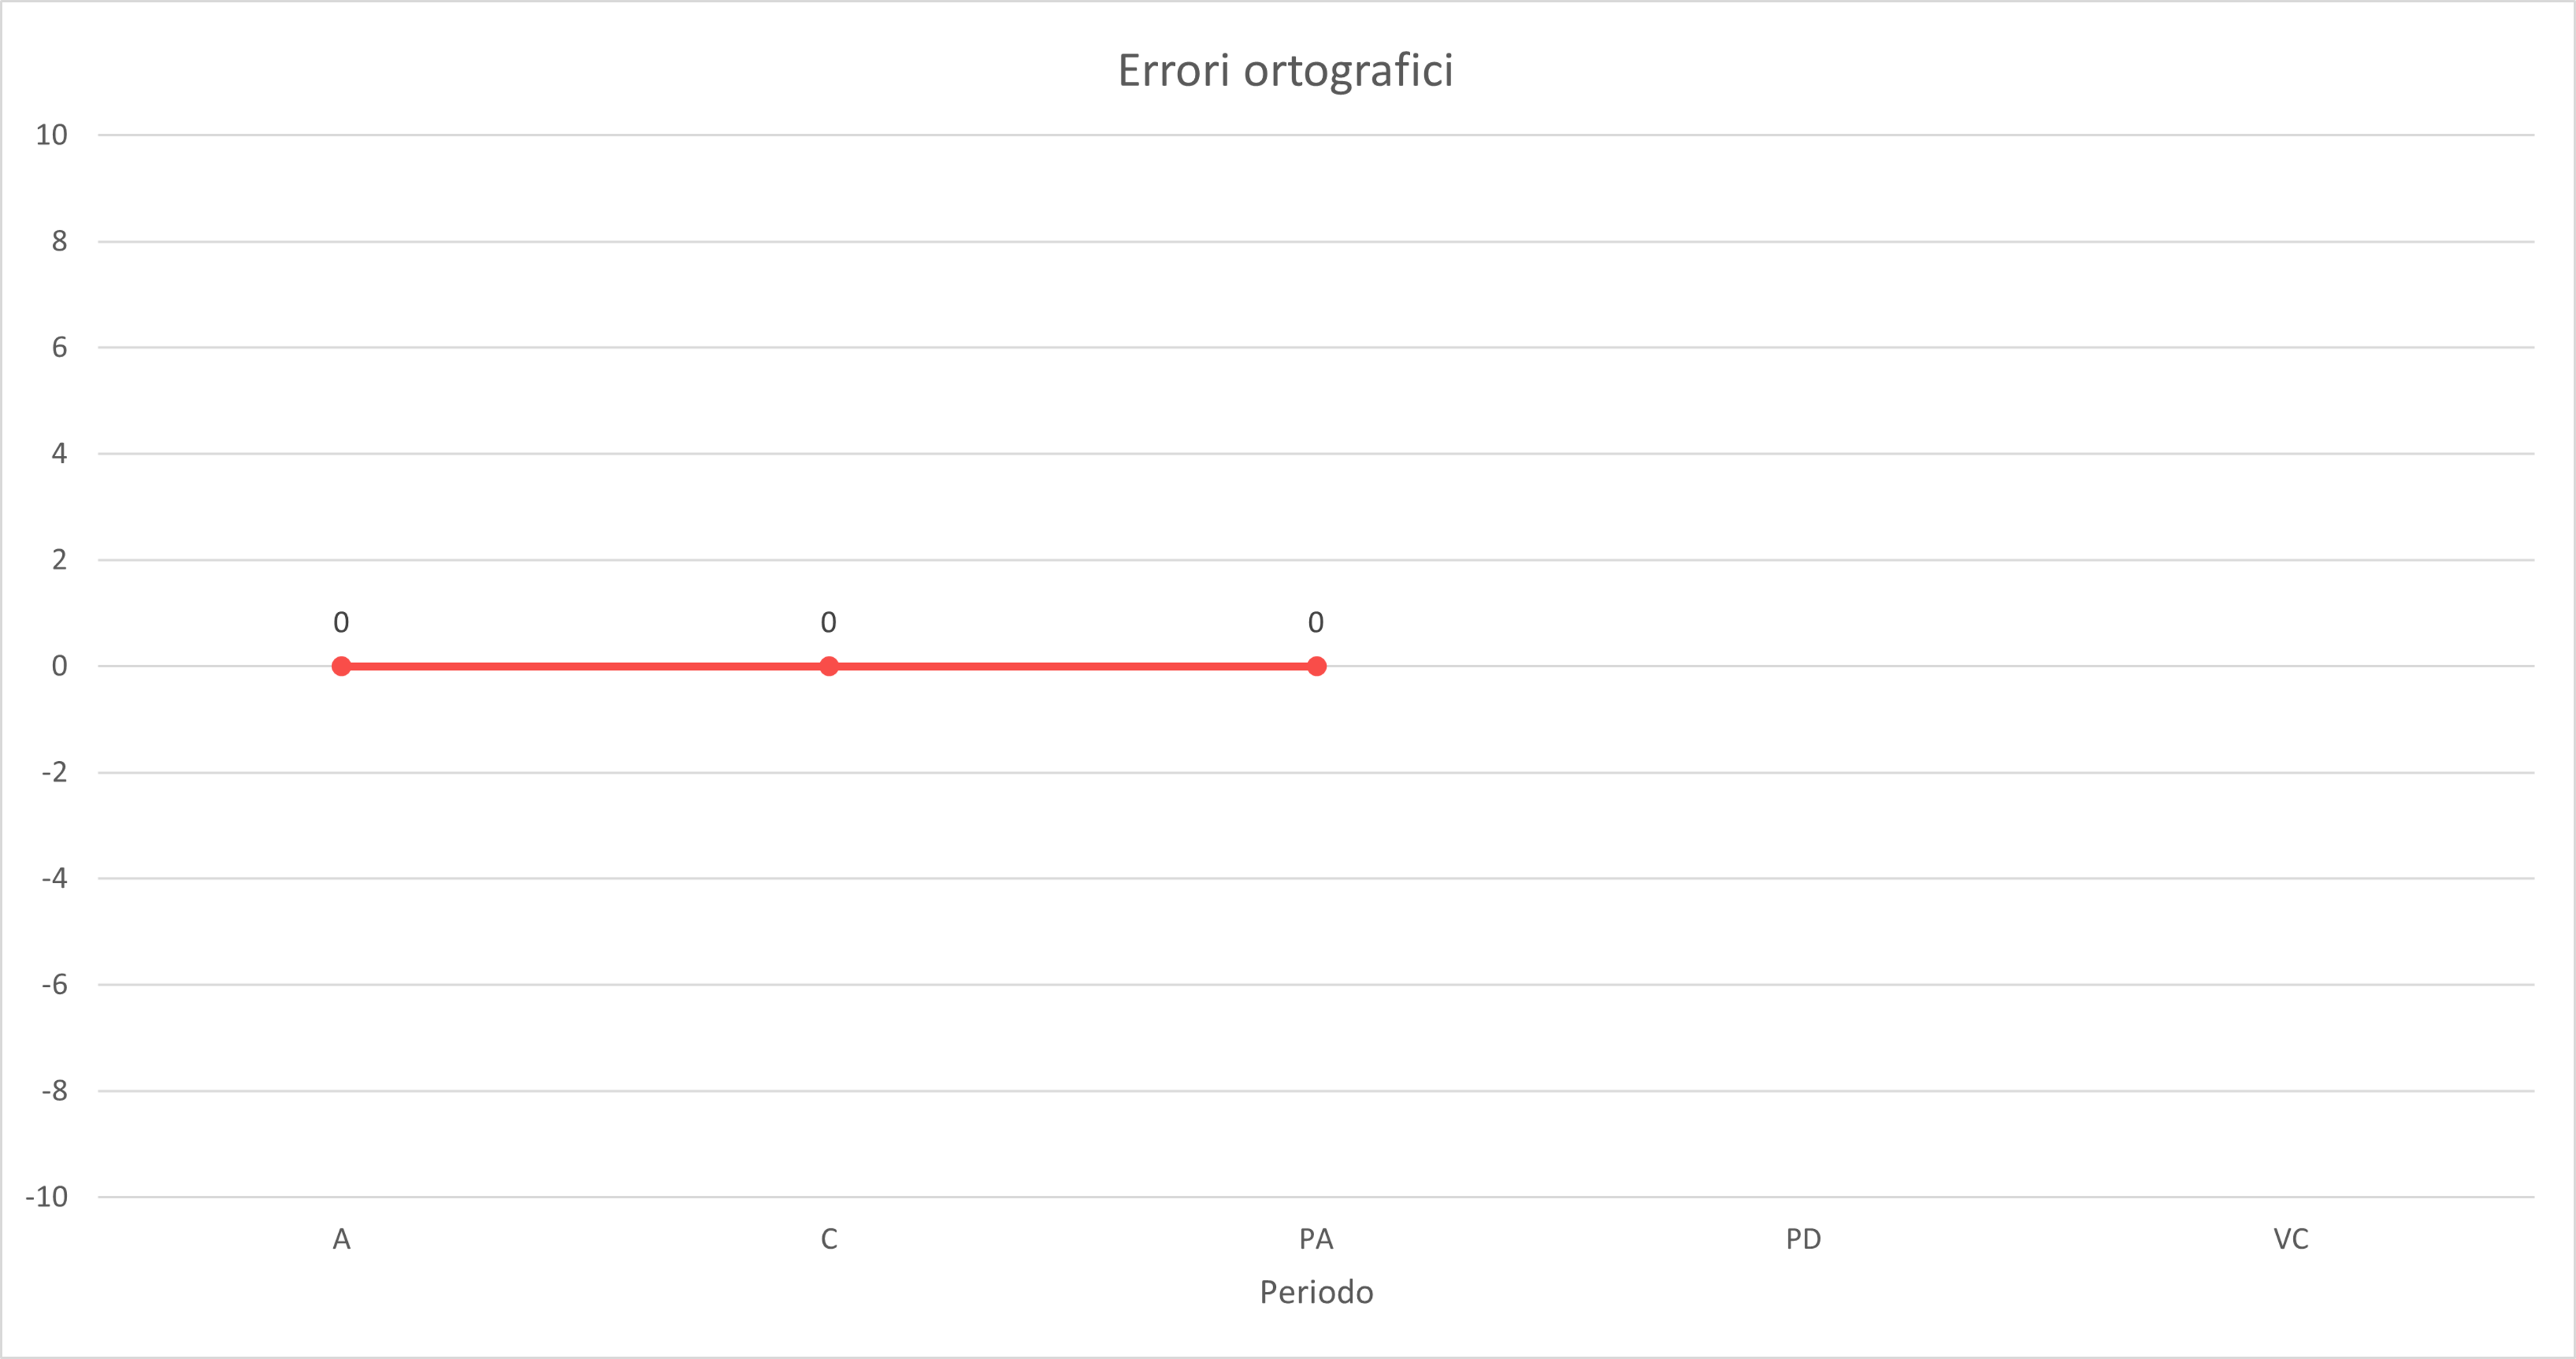
\includegraphics[scale=0.5]{sezioni/immagini/CorrettezzaOrtografica.png}
    \centering
\end{figure}
\subsubsection{MPR05 - PMS (Percentuale di metriche soddisfatte)}
\begin{figure}[!ht]
    \caption{Percentuale di metriche soddisfatte}
    \vspace{10px}
    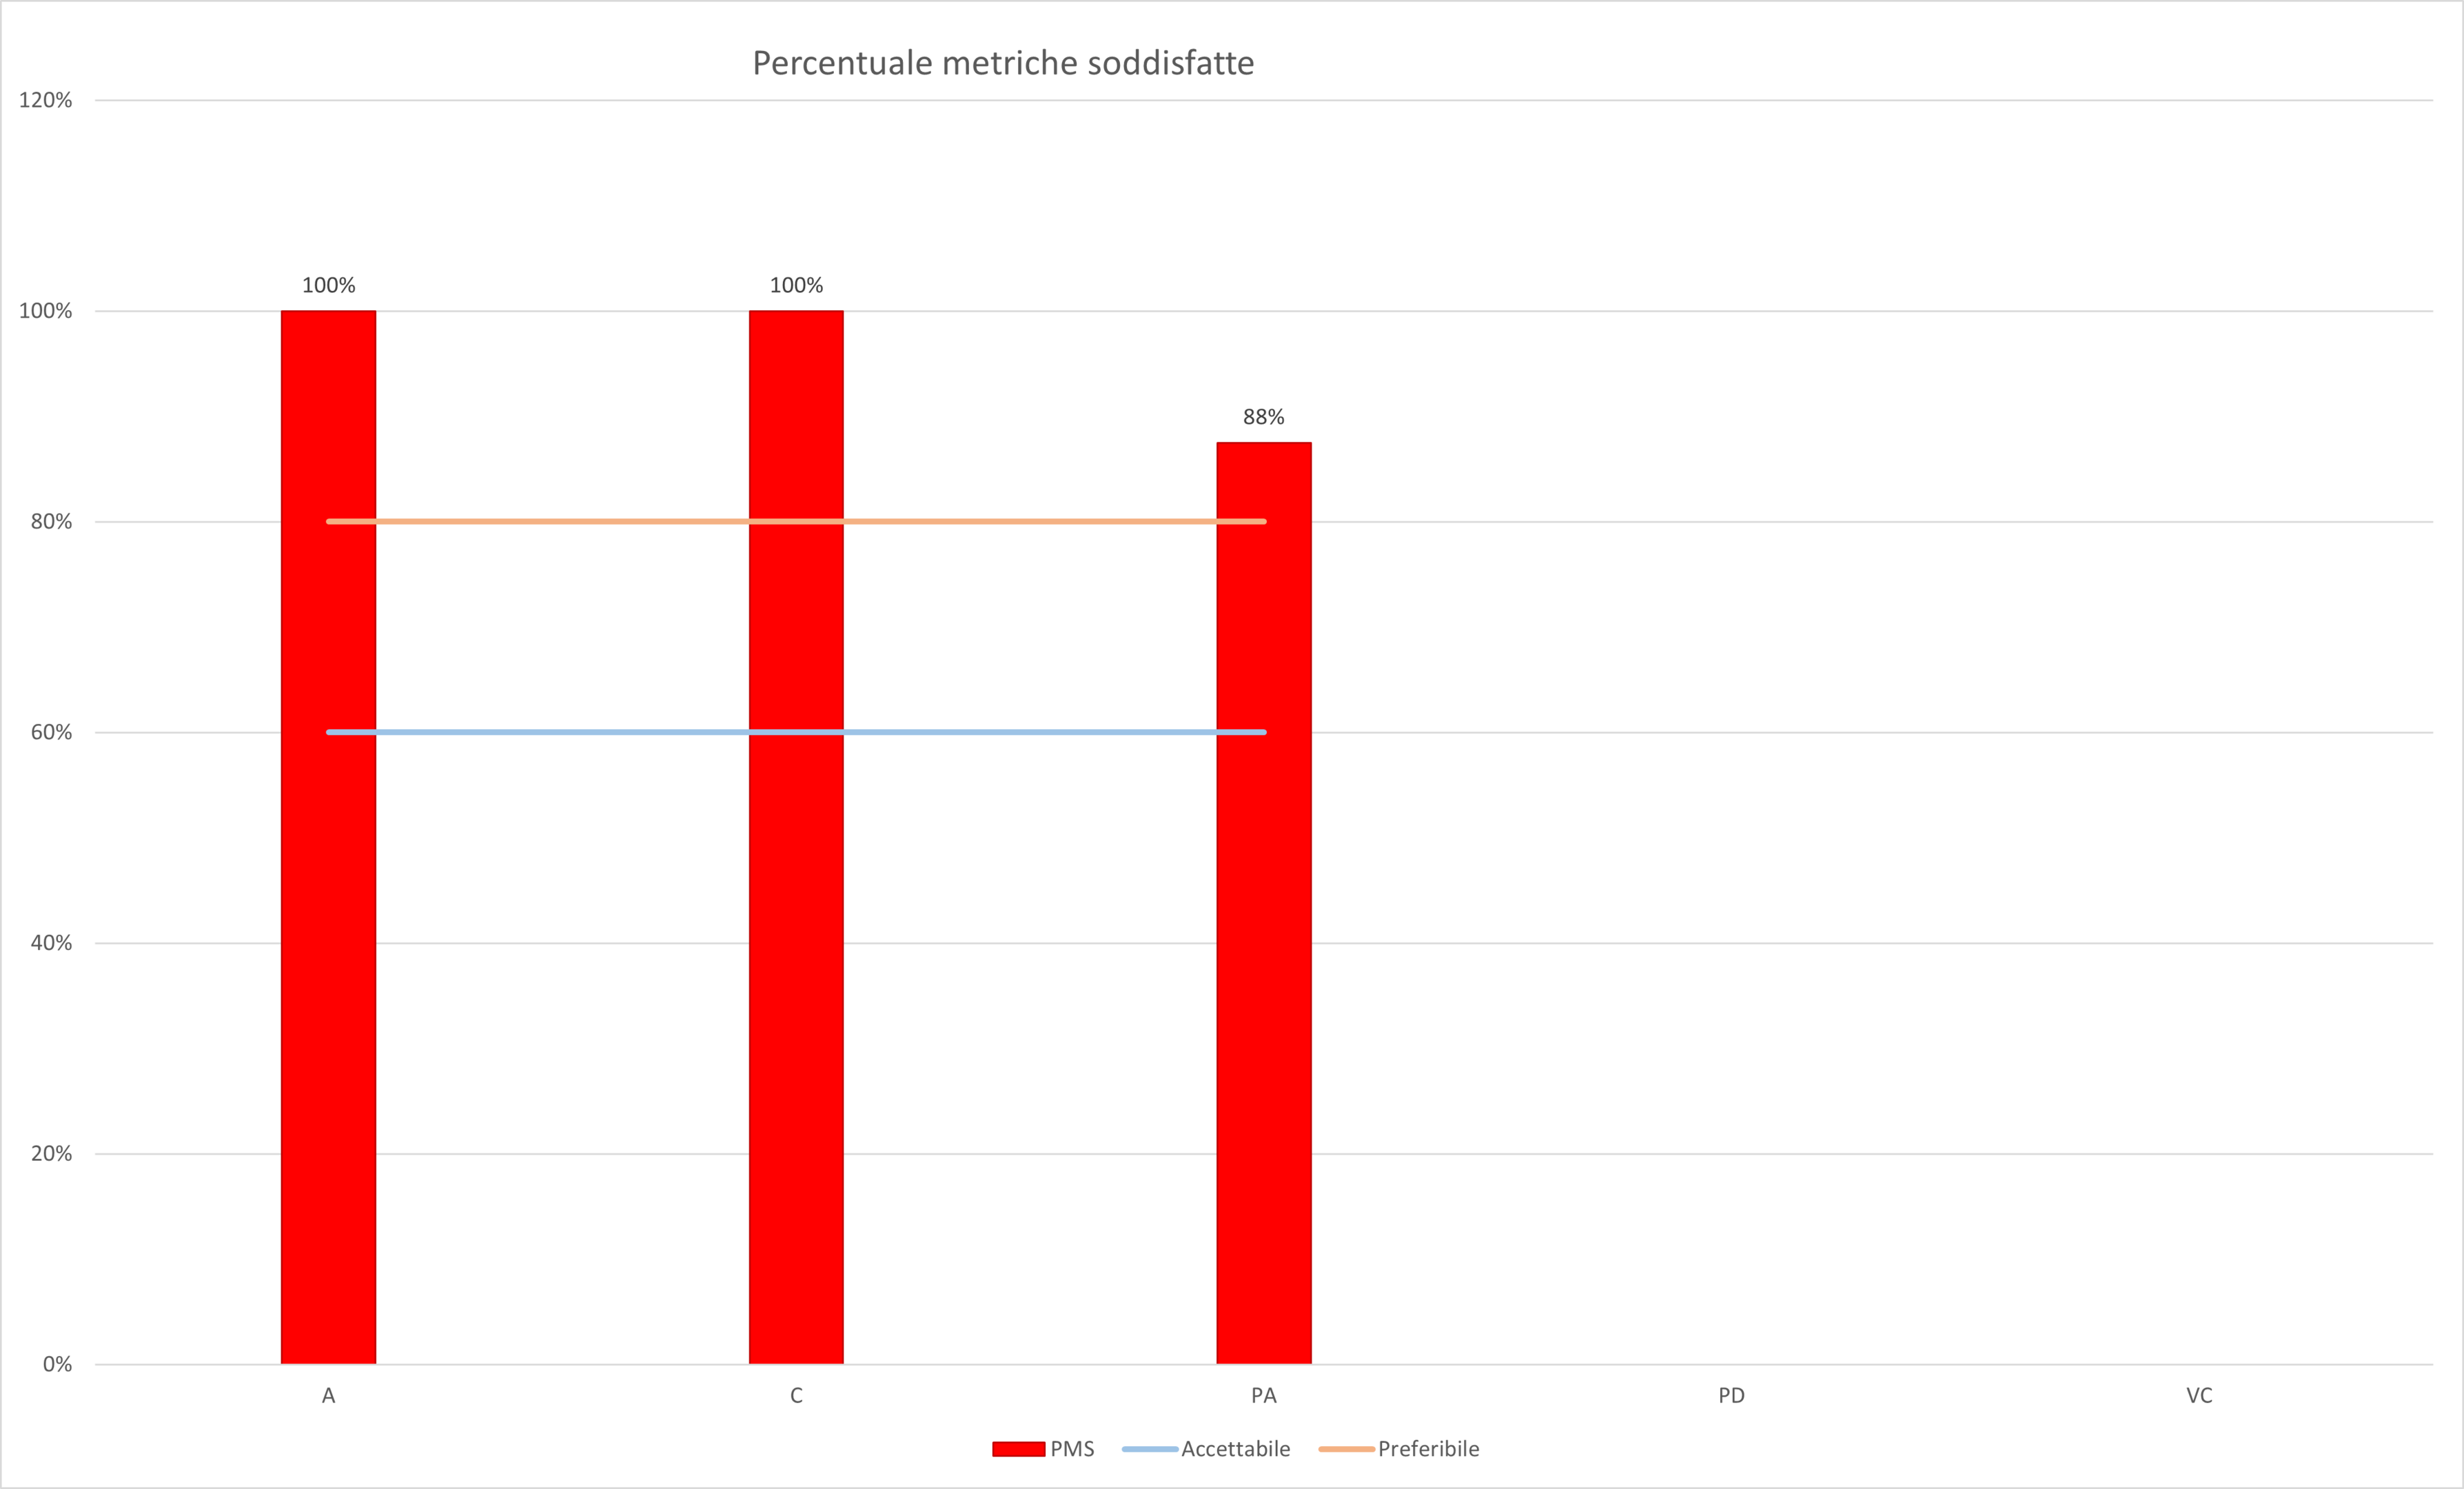
\includegraphics[scale=0.5]{sezioni/immagini/MetricheSoddisfatte.png}
    \centering
\end{figure}
\newpage
\subsubsection{MPR06 - CC (Code Coverage)}
\begin{figure}[!ht]
    \caption{Code Coverage}
    \vspace{10px}
    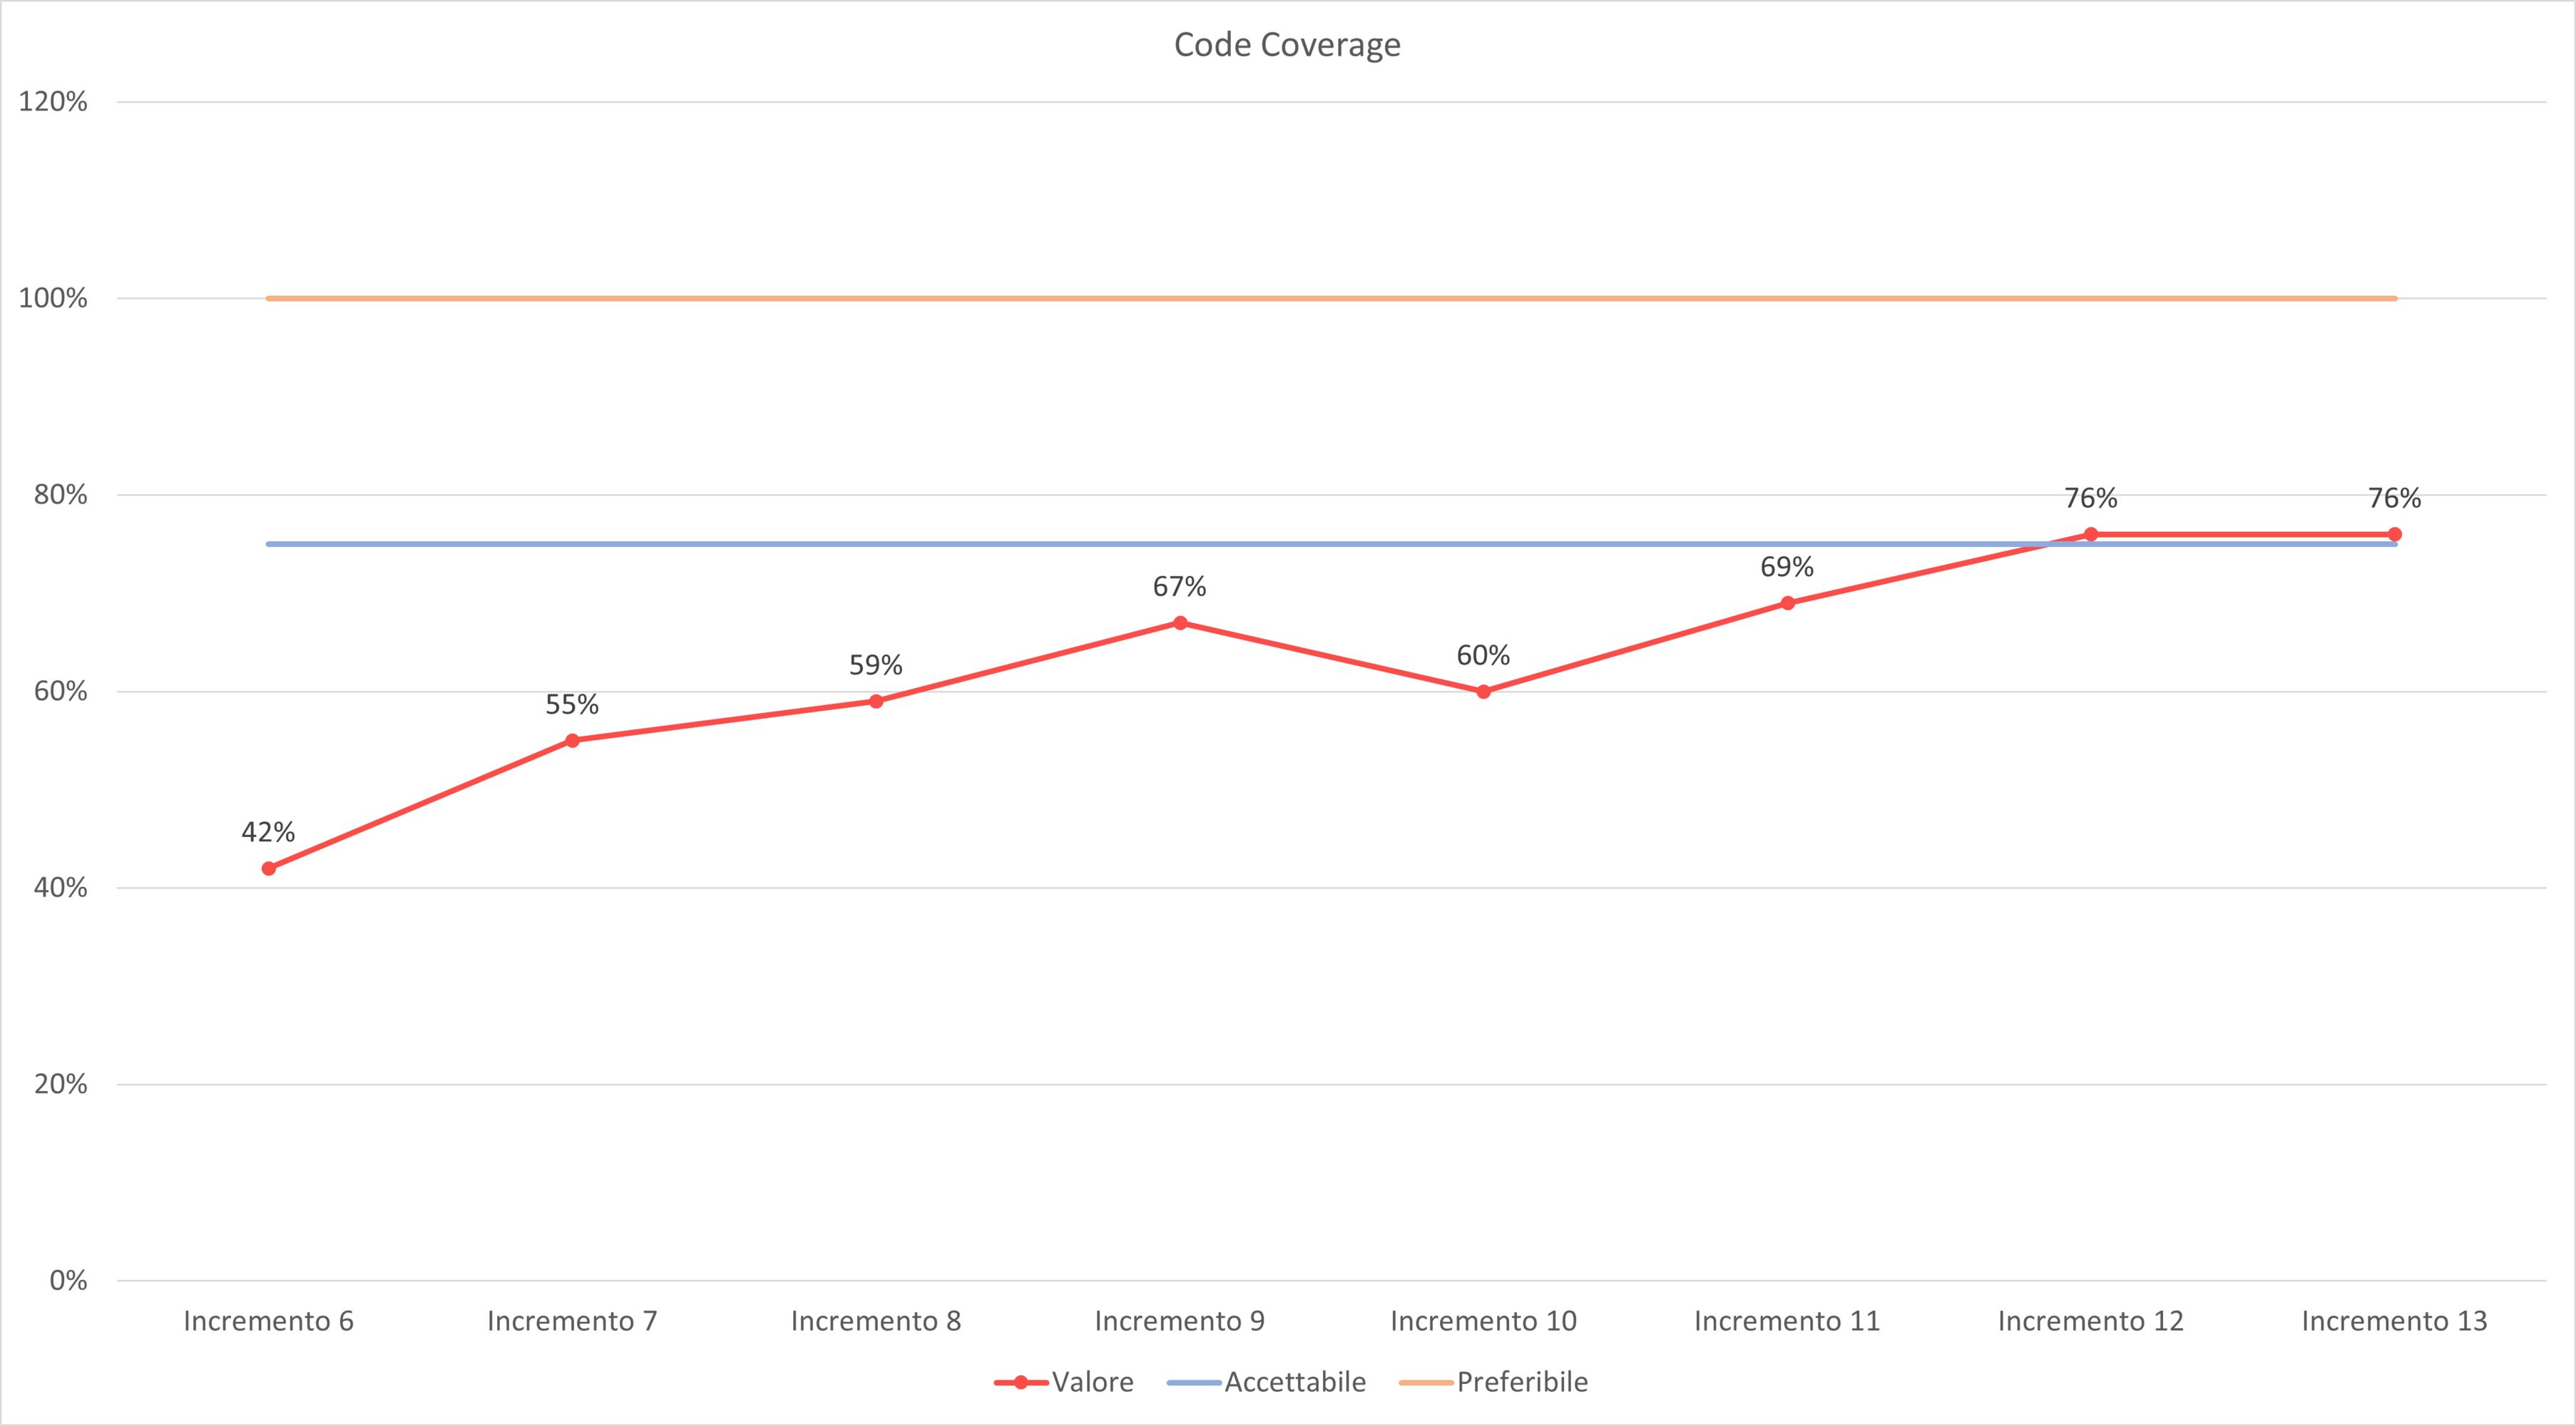
\includegraphics[scale=0.5]{sezioni/immagini/CodeCoverage.png}
    \centering
\end{figure}
\subsubsection{MPR07 - EAC (Estimate at Completion)}
\begin{figure}[!ht]
    \caption{Estimate at Completion}
    \vspace{10px}
    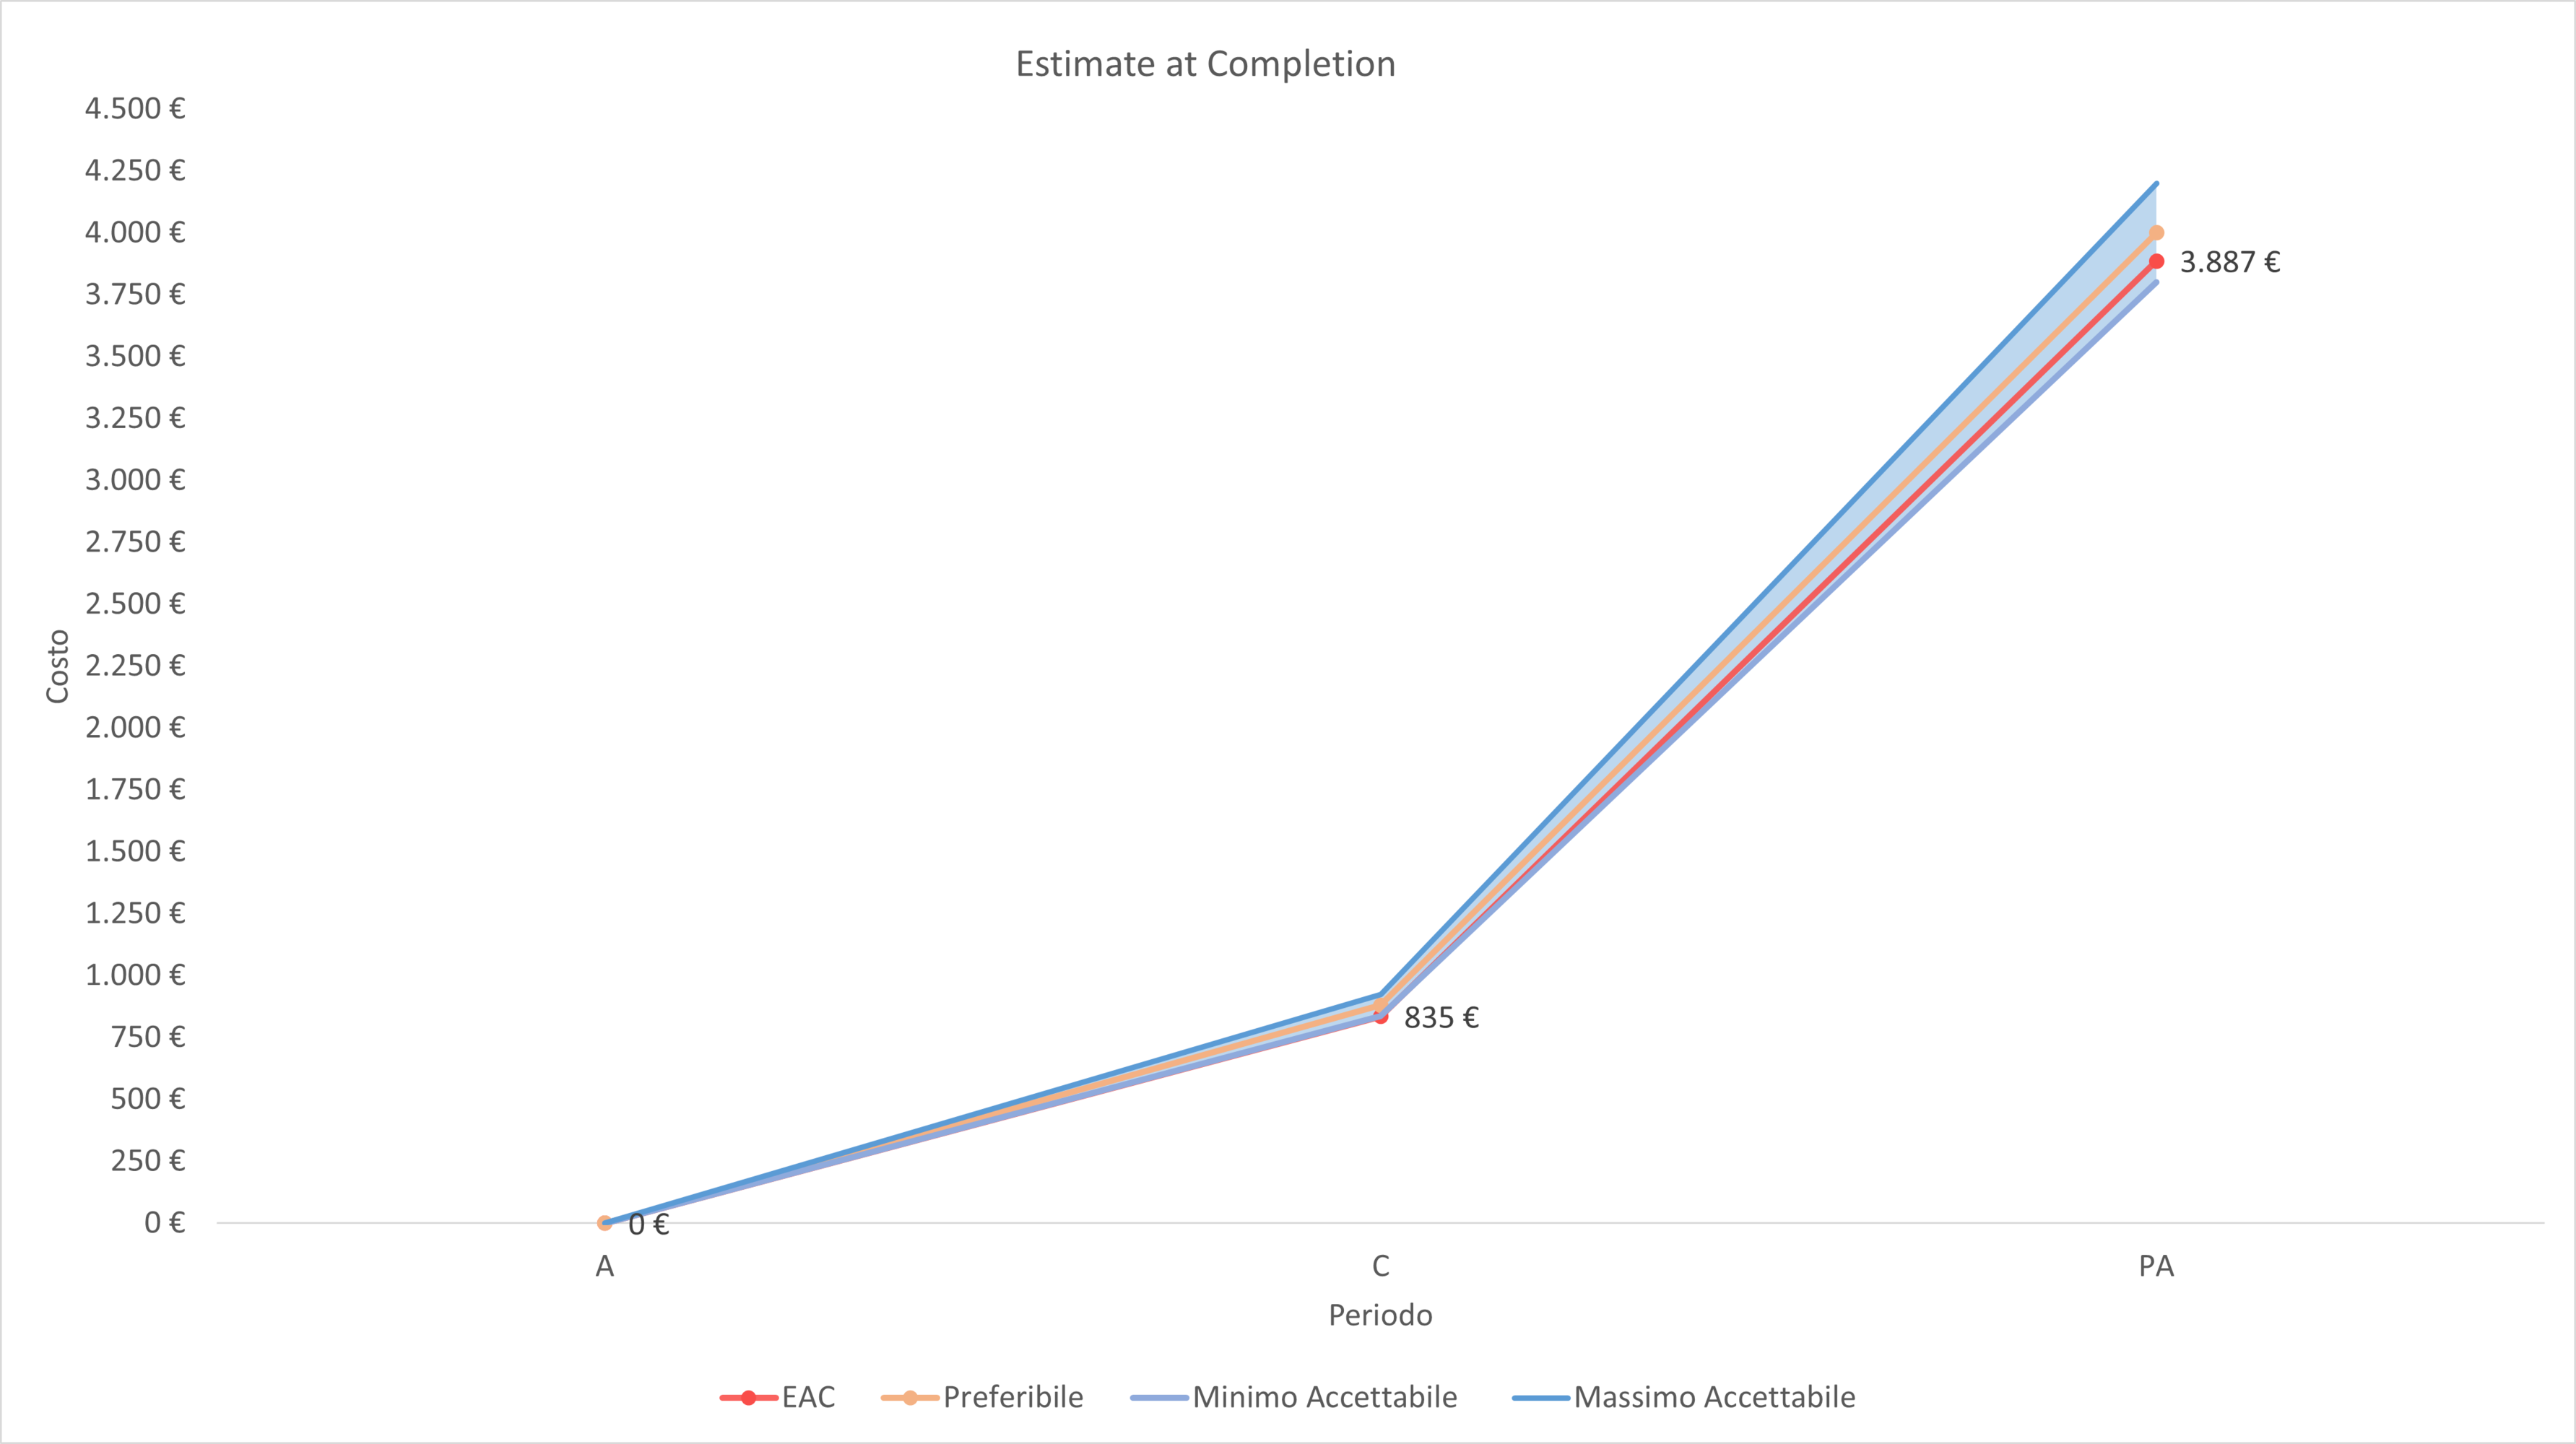
\includegraphics[scale=0.5]{sezioni/immagini/EstimateAtCompletion.png}
    \centering
\end{figure}
\pagebreak
\subsubsection{MPR08 - VAC (Variance at Completion)}
\begin{figure}[!ht]
    \caption{Variance at Completion}
    \vspace{10px}
    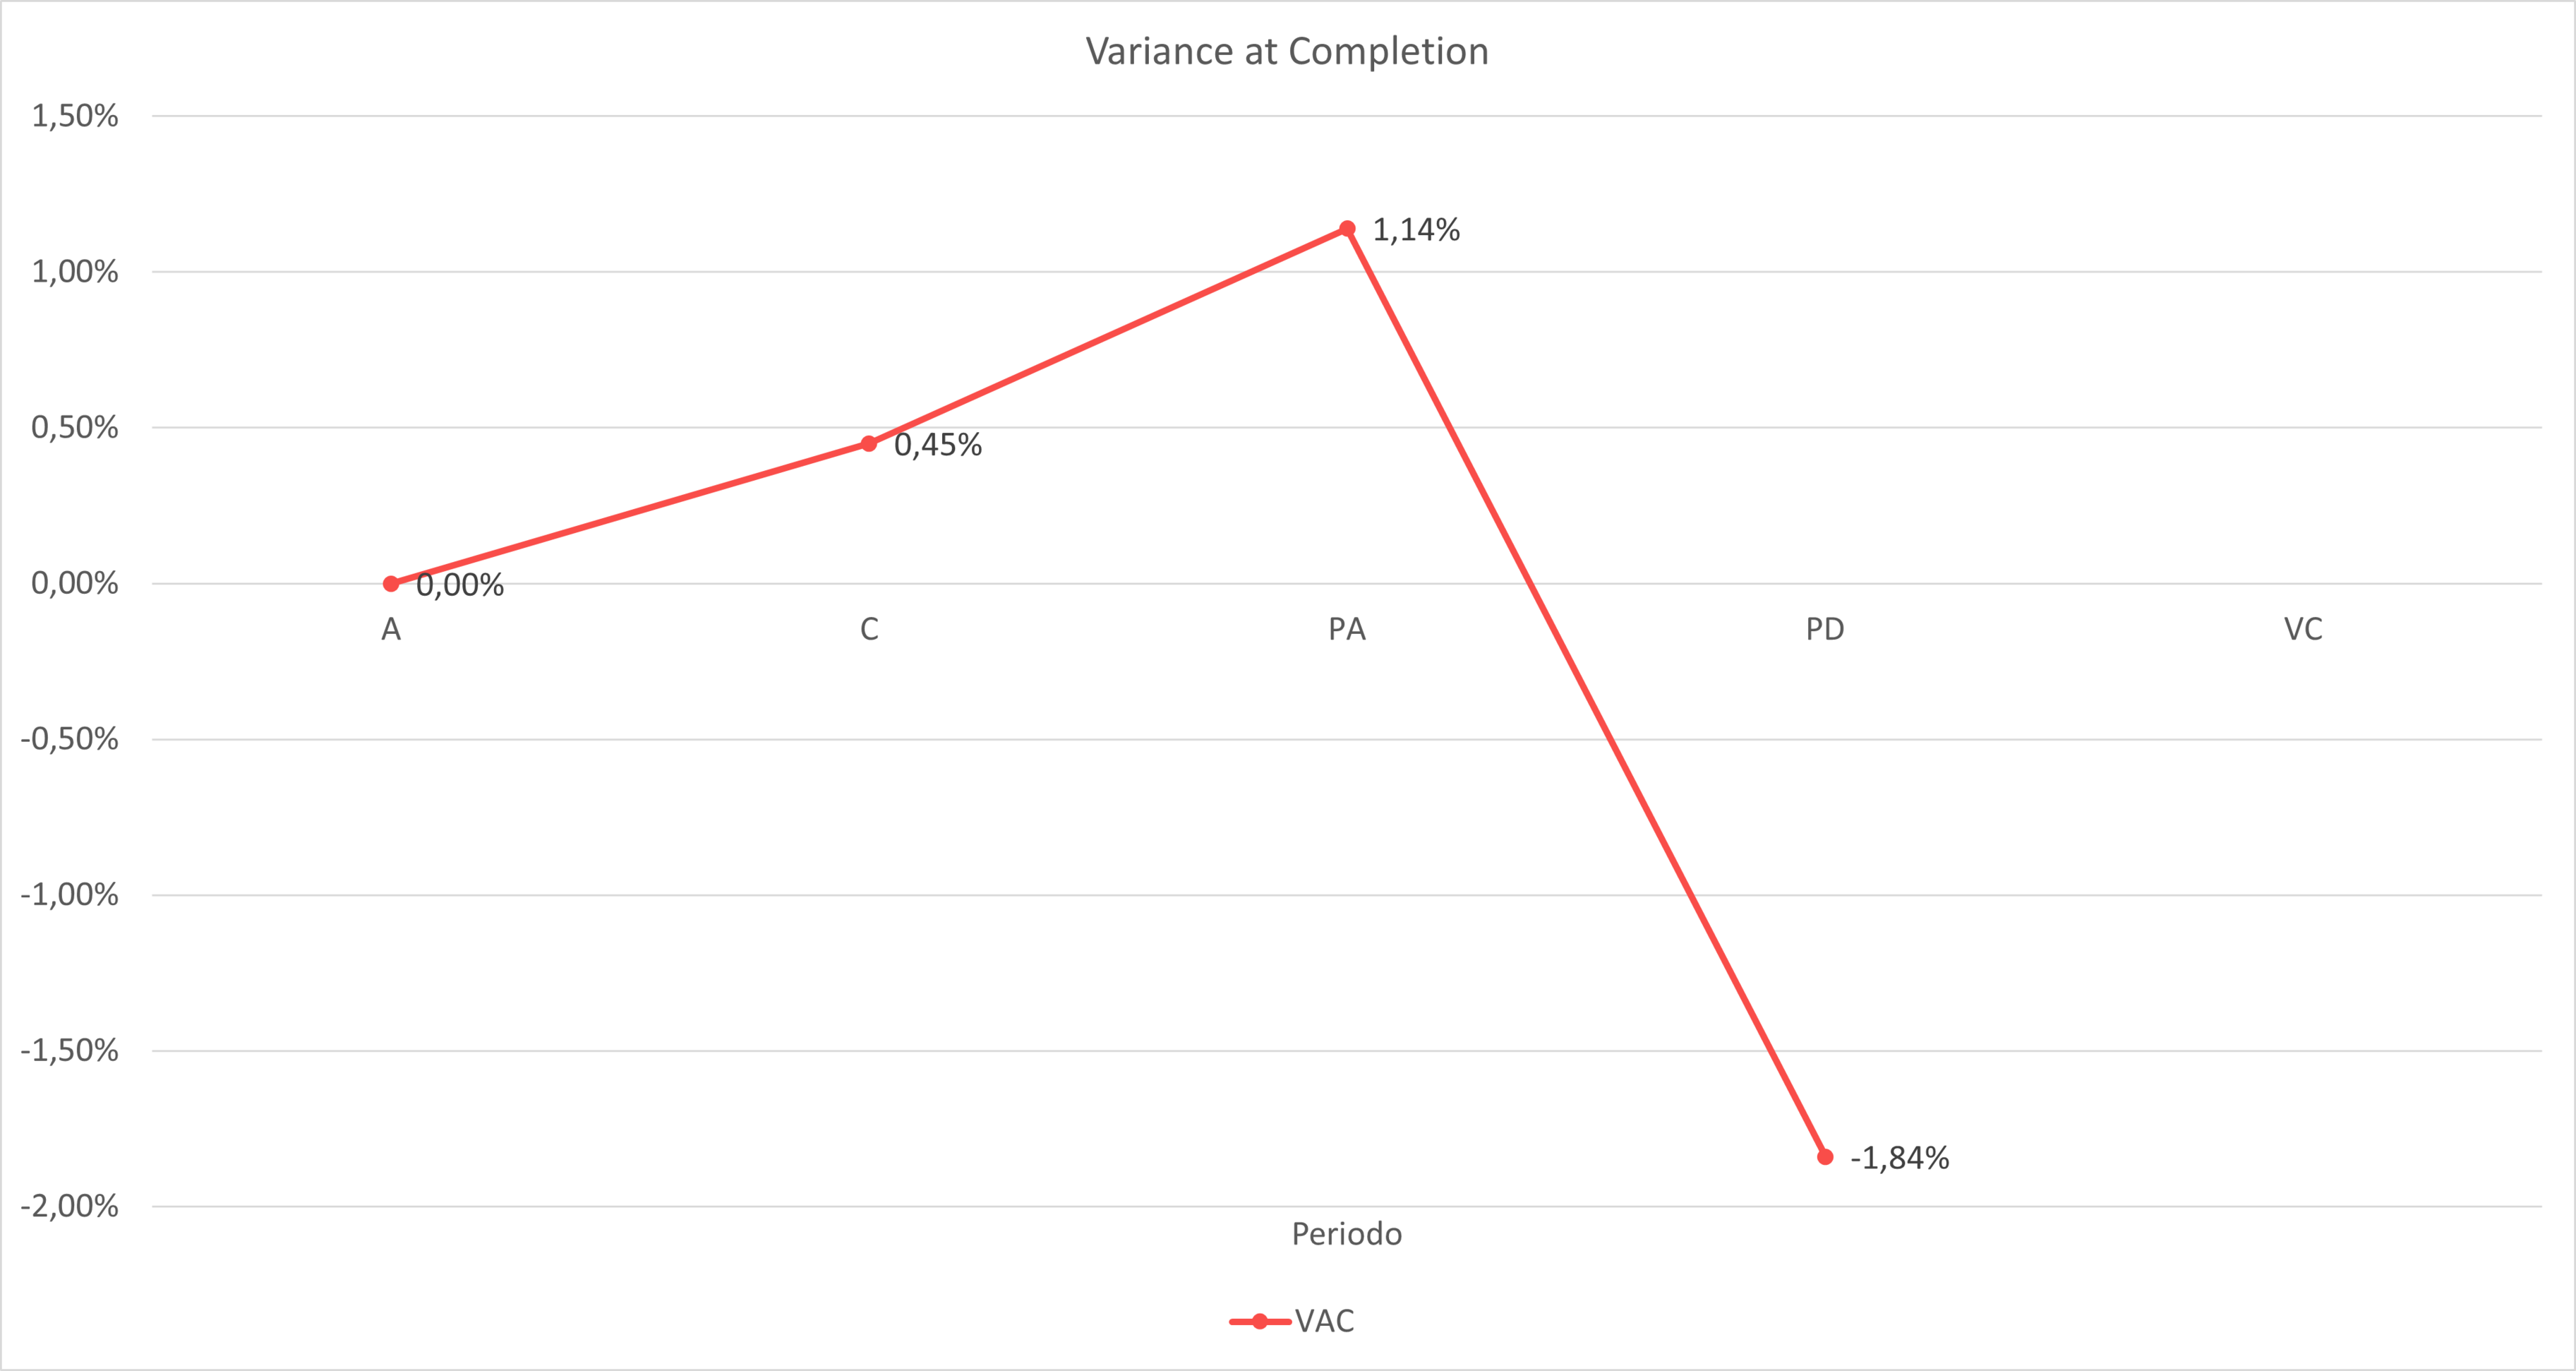
\includegraphics[scale=0.5]{sezioni/immagini/VarianceAtCompletion.png}
    \centering
\end{figure}
\subsubsection{MPR09 - AC (Actual Cost)}
\begin{figure}[!ht]
    \caption{Actual Cost}
    \vspace{10px}
    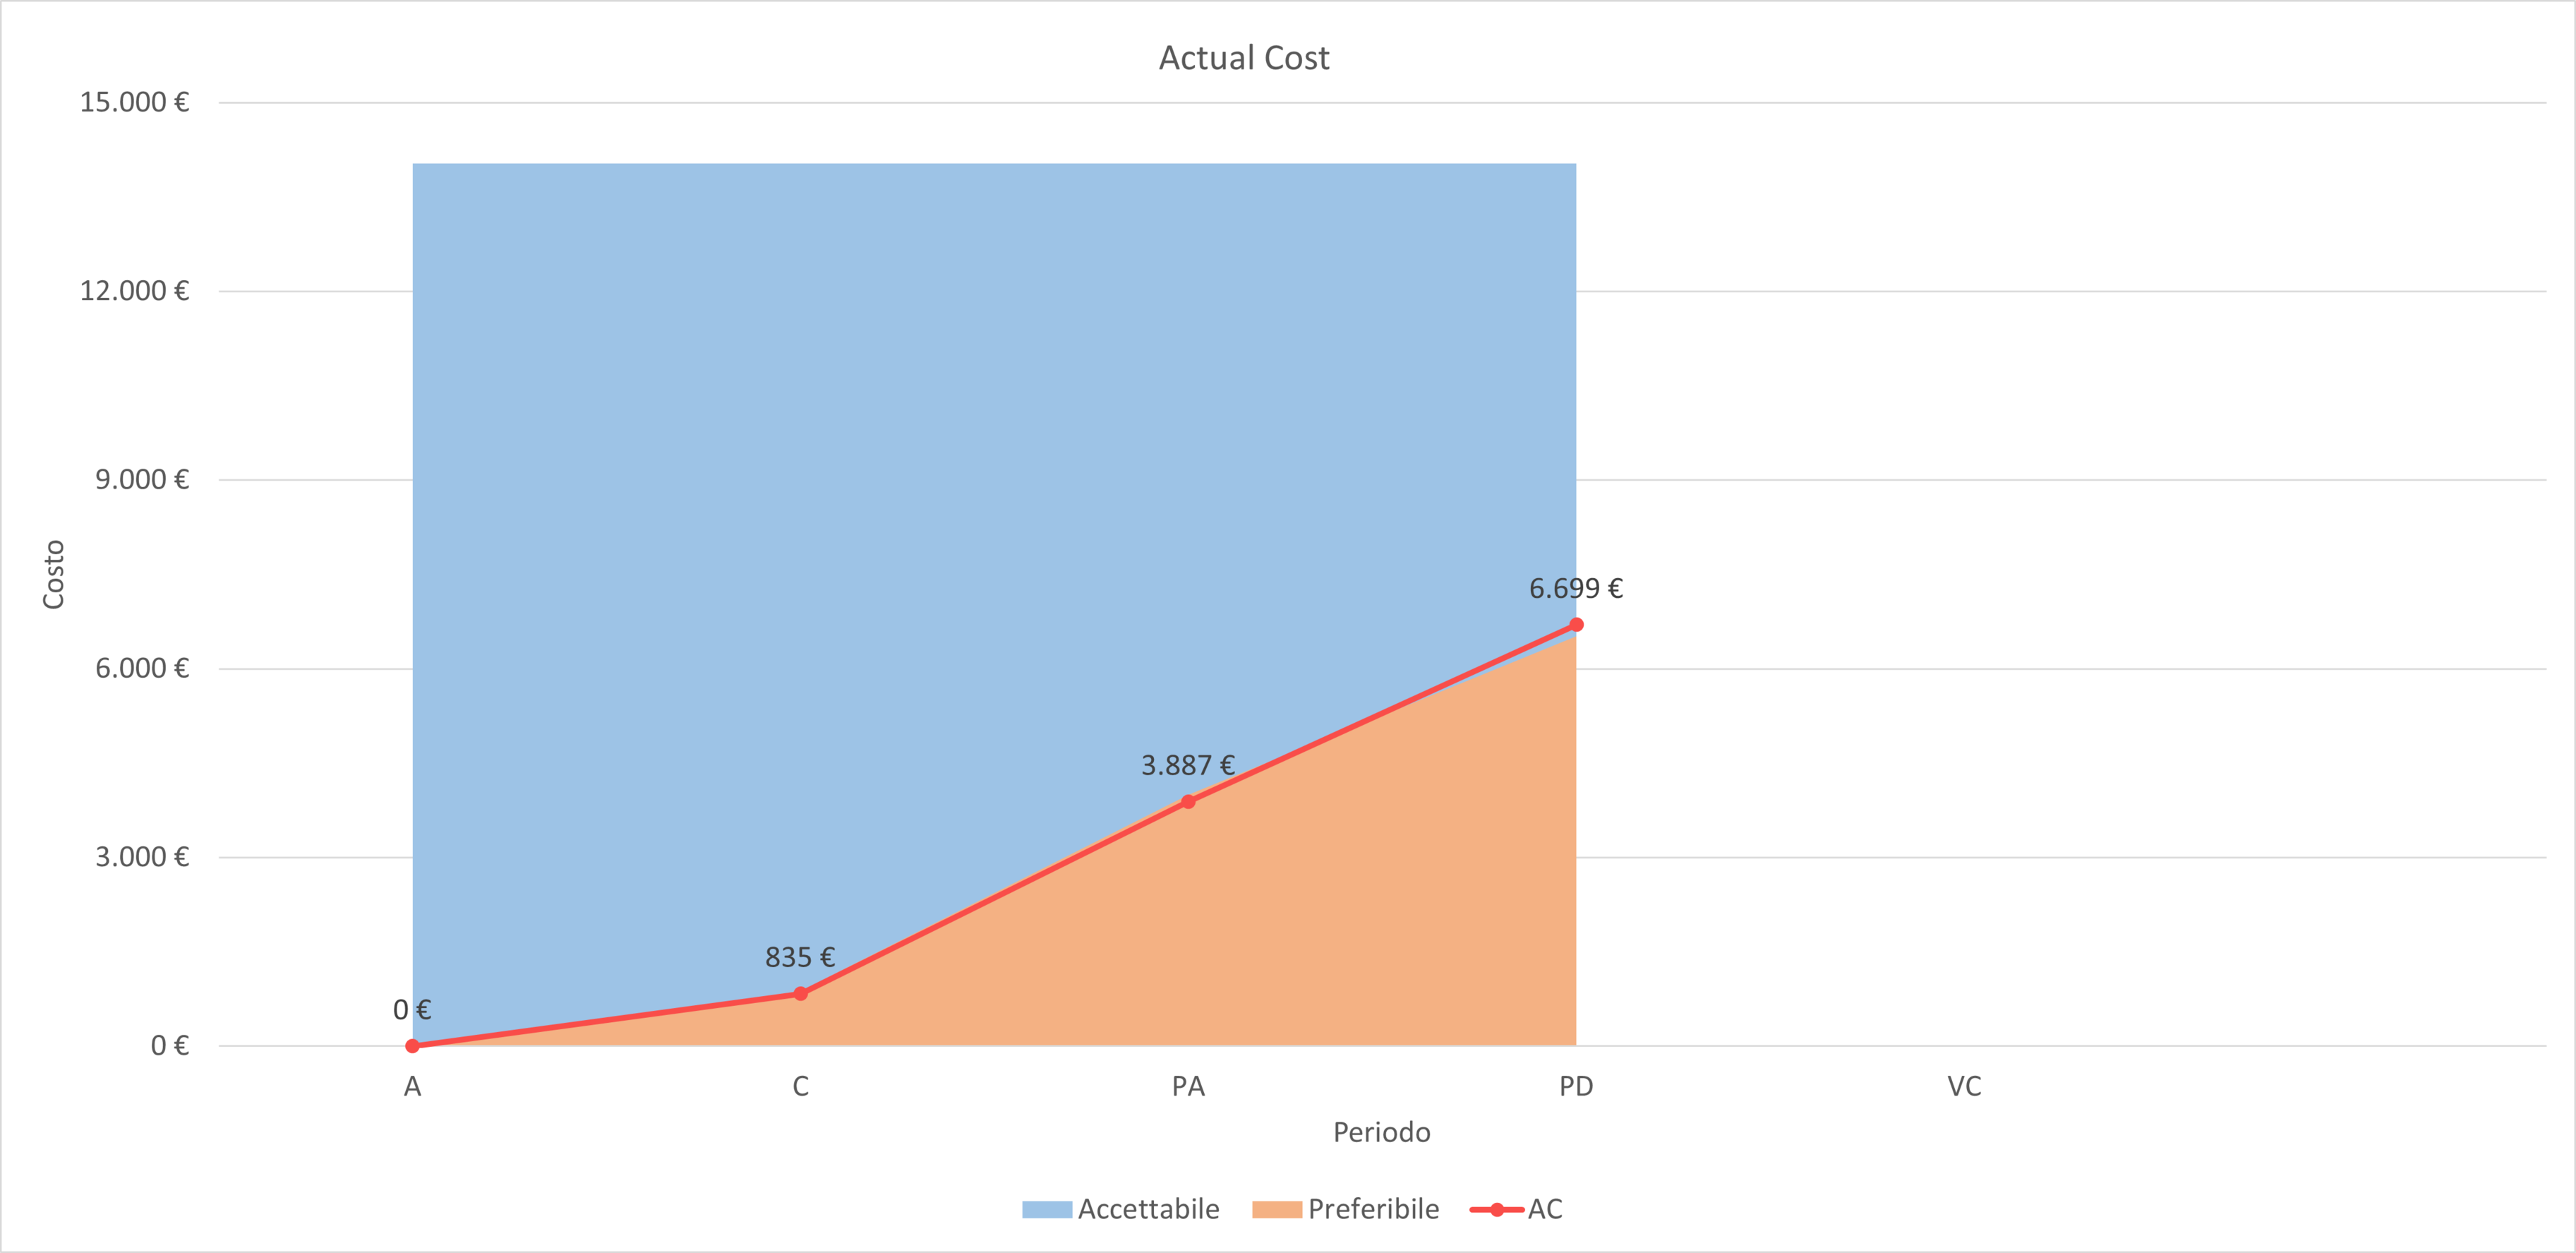
\includegraphics[scale=0.5]{sezioni/immagini/ActualCost.png}
    \centering
\end{figure}
\pagebreak
\subsubsection{MPR10 - SV (Schedule Variance)}
\begin{figure}[!ht]
    \caption{Schedule Variance}
    \vspace{10px}
    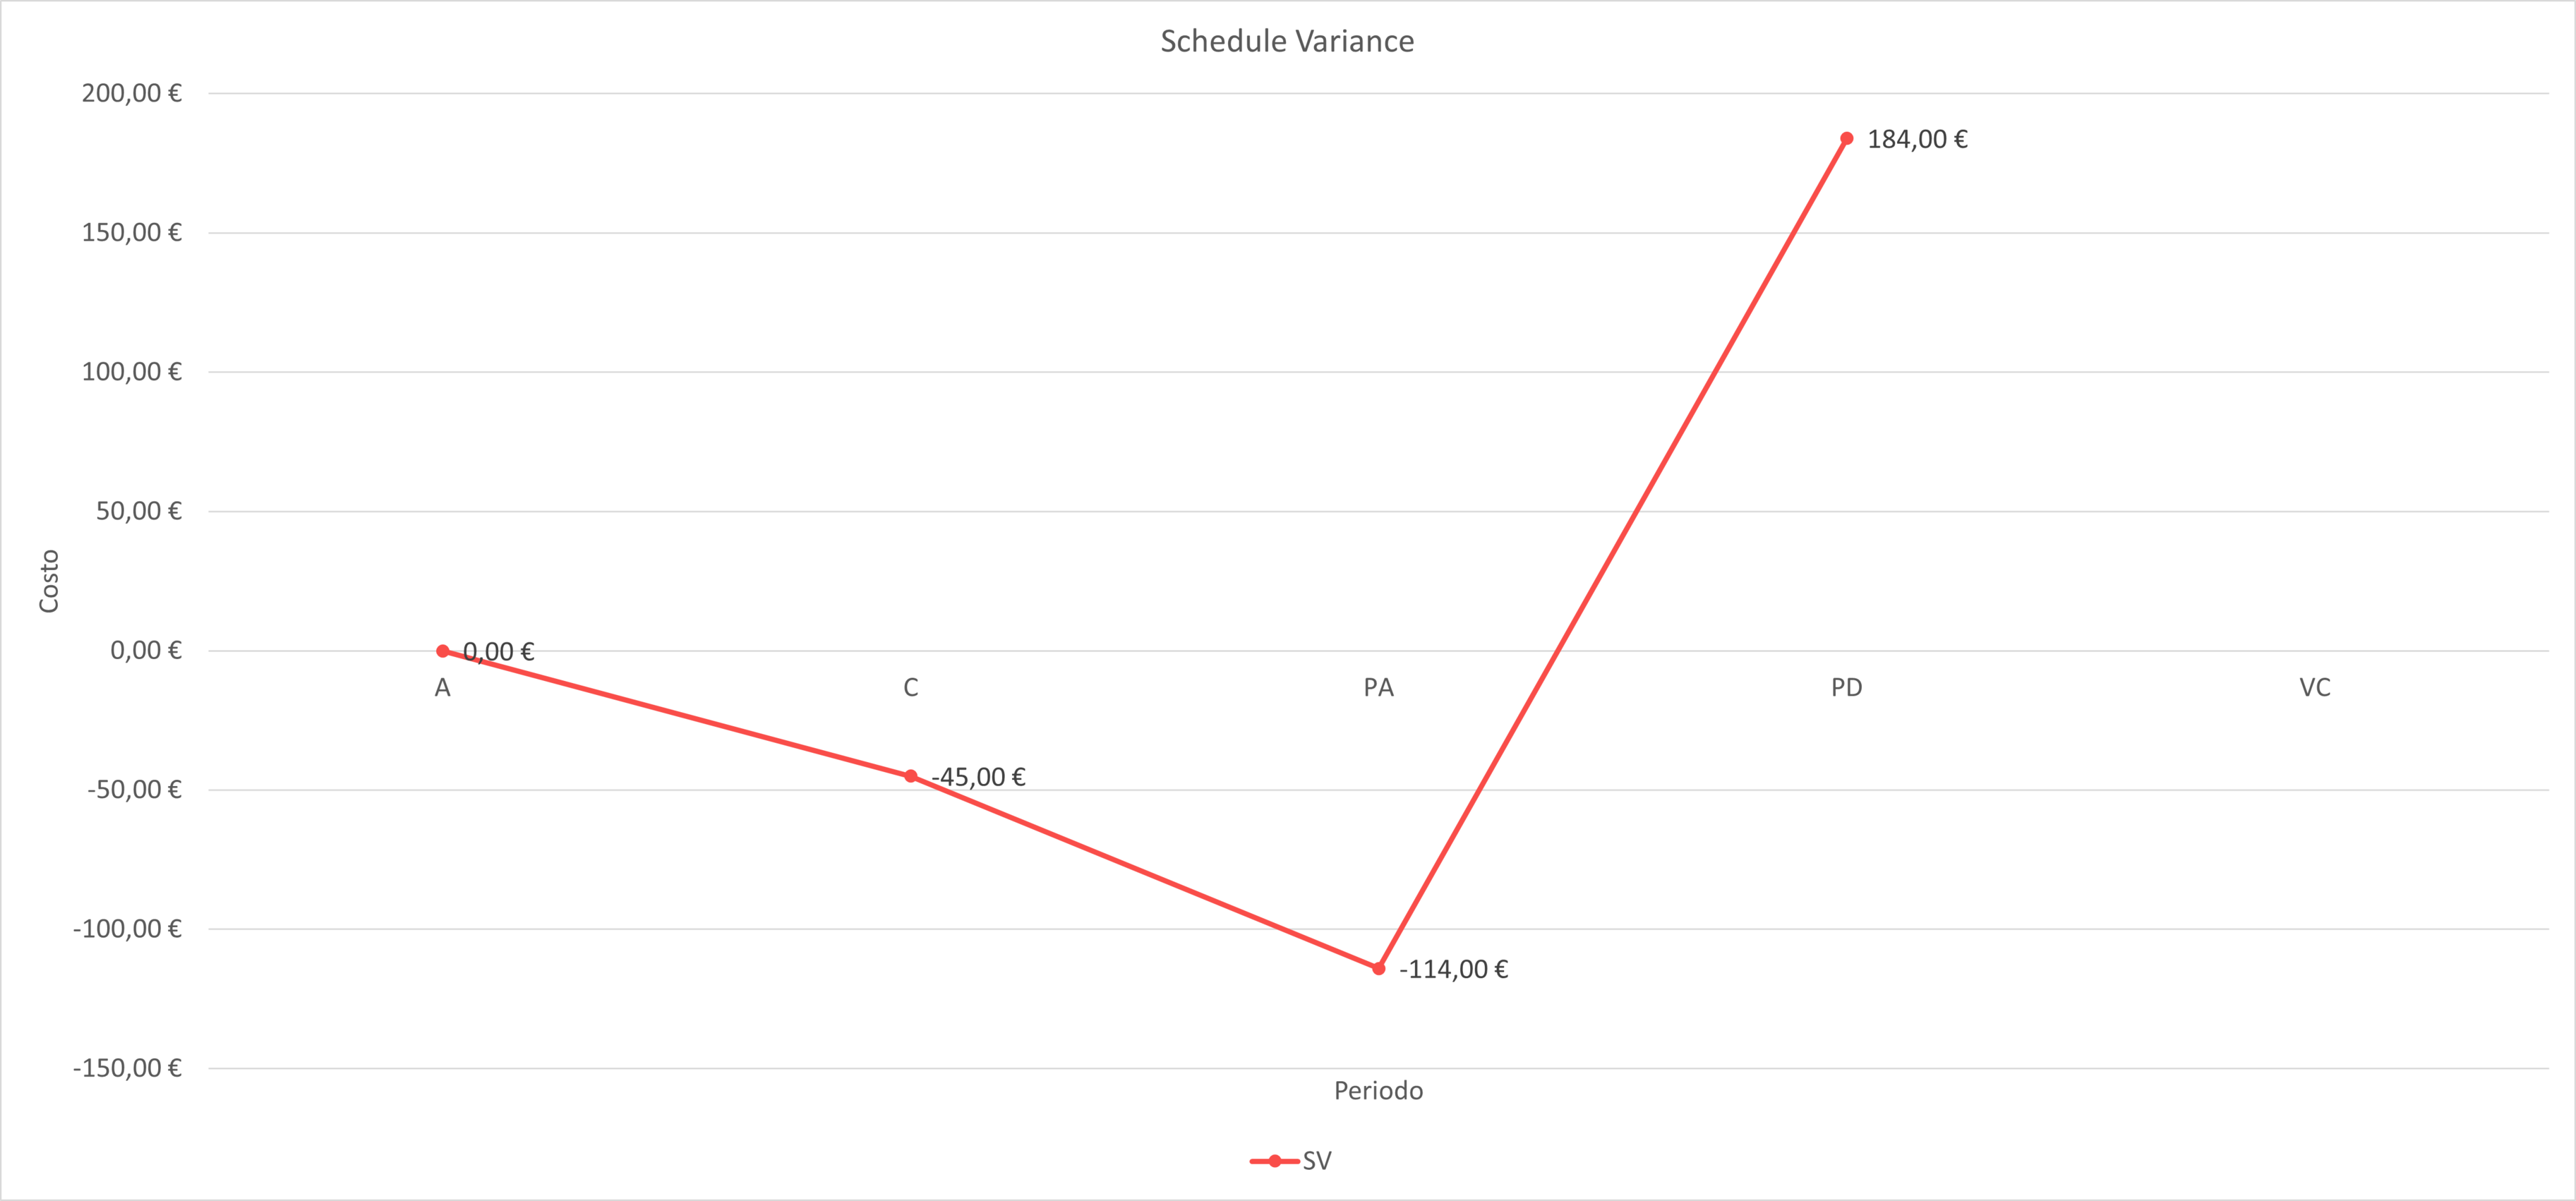
\includegraphics[scale=0.5]{sezioni/immagini/ScheduleVariance.png}
    \centering
\end{figure}
\subsubsection{MPR11 - BV (Budget Variance)}
\begin{figure}[!ht]
    \caption{Budget Variance}
    \vspace{10px}
    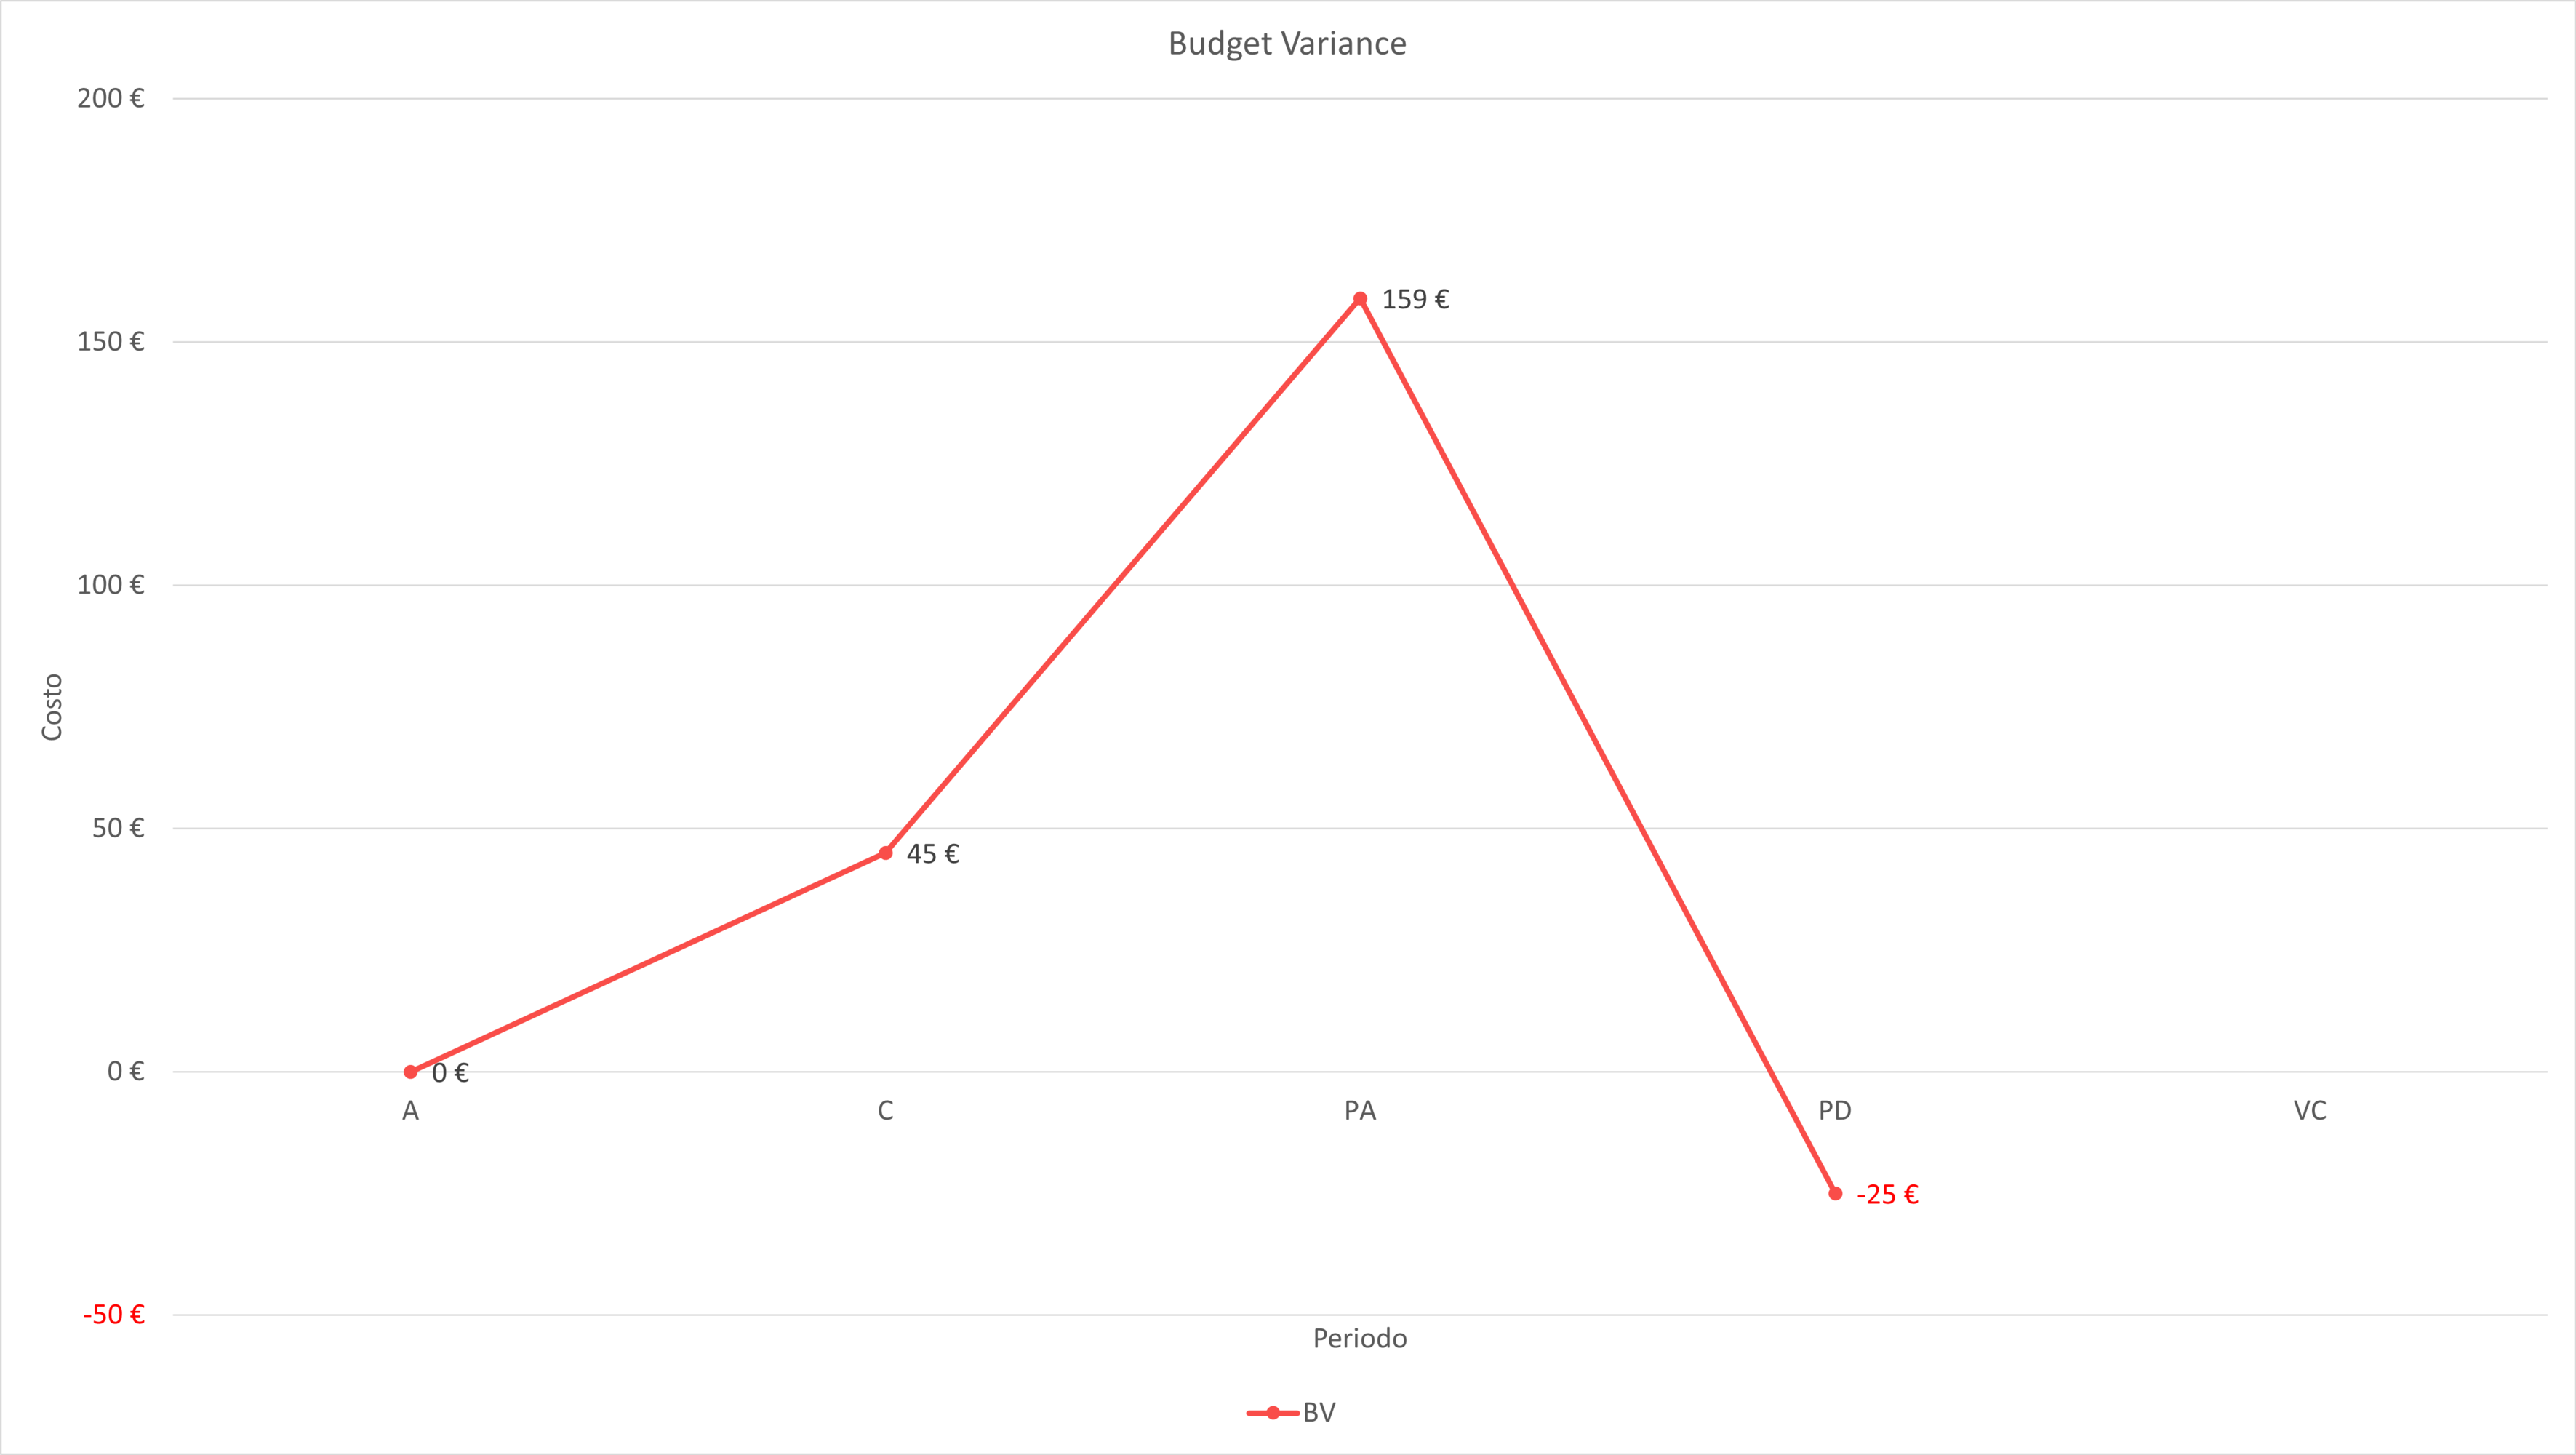
\includegraphics[scale=0.5]{sezioni/immagini/BudgetVariance.png}
    \centering
\end{figure}
\pagebreak
\subsubsection{MPD01 - Percentuale Test Superati}
\begin{figure}[!ht]
    \caption{Percentuale Test Superati}
    \vspace{10px}
    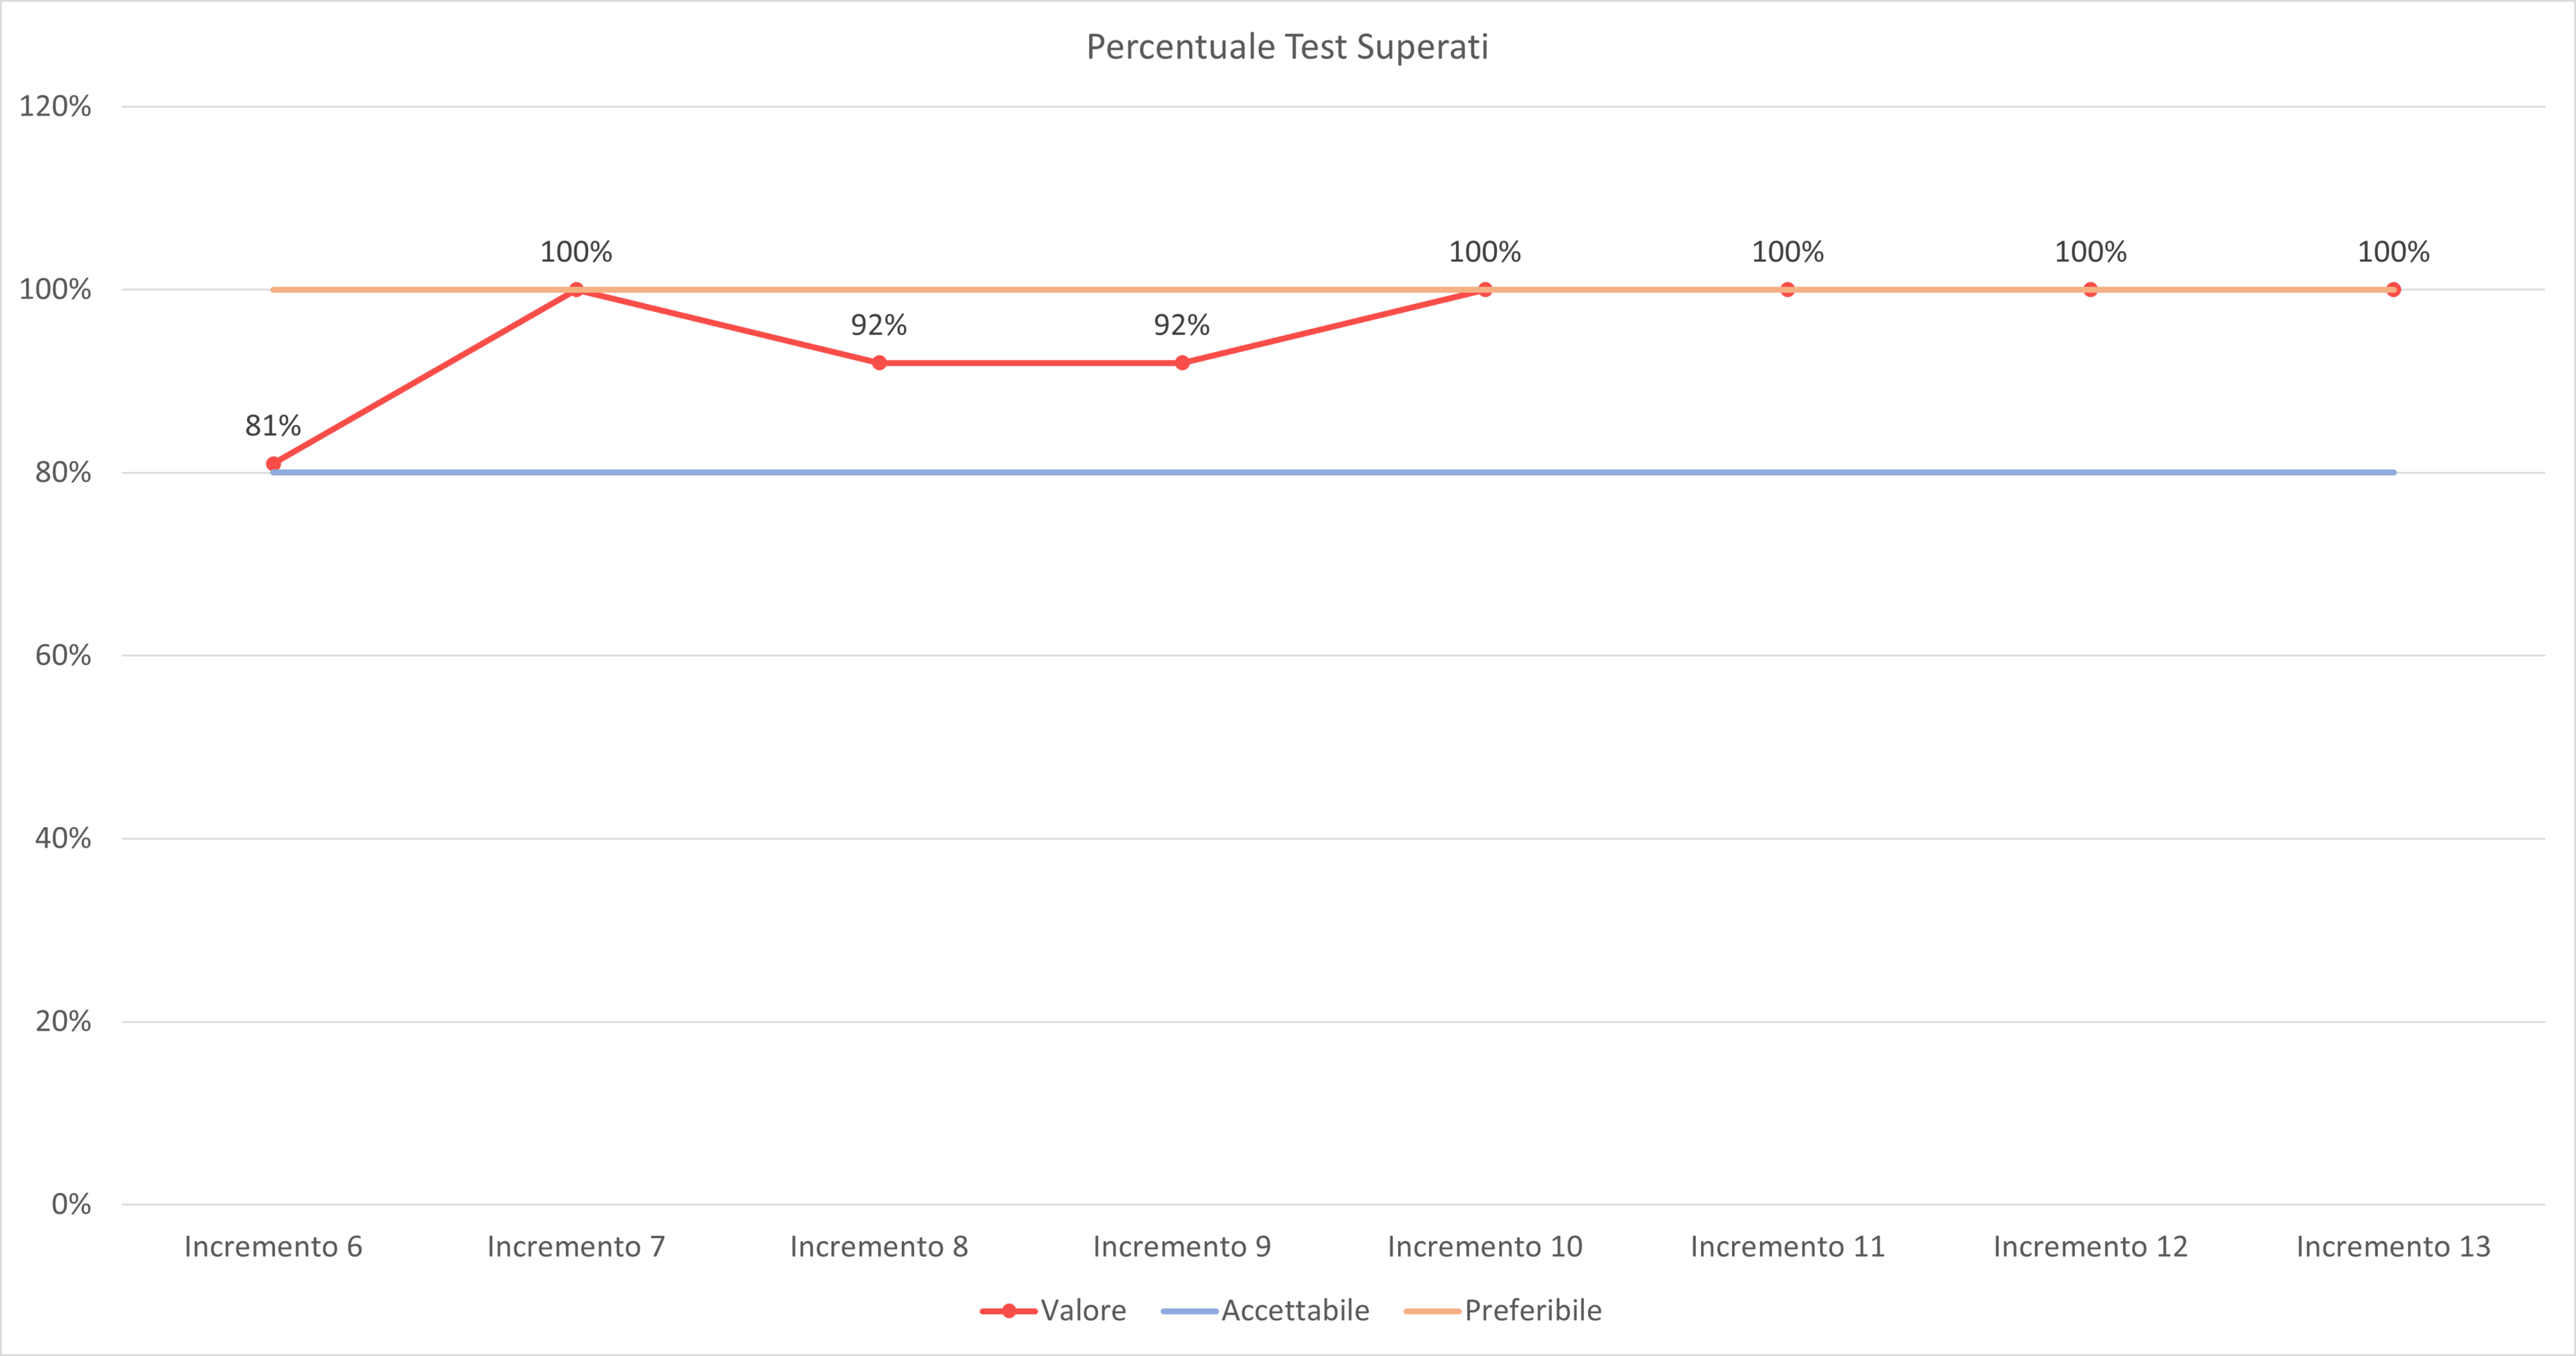
\includegraphics[scale=0.5]{sezioni/immagini/PercentualeTestSuperati.png}
    \centering
\end{figure}
\subsubsection{MPD02 - Densità errori}
\begin{figure}[!ht]
    \caption{Densità errori}
    \vspace{10px}
    \includegraphics[scale=0.5]{sezioni/immagini/DensitàErrori.png}
    \centering
\end{figure}
\pagebreak
\subsubsection{MPD03 - Facilità di utilizzo}
Per il calcolo di questa metrica si è tenuto in considerazione il segunte percorso:\\
Home -> lista dei prodotti -> prodotto -> carrello -> checkout.\\
Poichè durante i primi due incrementi il numero delle funzionalità offerte erano esigue e l'interfaccia utente era molto più semplice,
il numero di click per raggiungere il checkout era minore.
\begin{figure}[!ht]
    \caption{Facilità di utilizzo}
    \vspace{10px}
    \includegraphics[scale=0.5]{sezioni/immagini/FacilitàUtilizzo.png}
    \centering
\end{figure}
\subsubsection{MPD04 - Facilità di apprendimento}
\begin{figure}[!ht]
    \caption{Facilità di apprendimento}
    \vspace{10px}
    \includegraphics[scale=0.5]{sezioni/immagini/FacilitàApprendimento.png}
    \centering
\end{figure}
\pagebreak
\subsubsection{MPD05 - Profondità della gerarchia}
\begin{figure}[!ht]
    \caption{Profondità della gerarchia}
    \vspace{10px}
    \includegraphics[scale=0.5]{sezioni/immagini/ProfonditàGerarchia.png}
    \centering
\end{figure}
\begin{figure}[!ht]
    \caption{Profondità della gerarchia - Utente non autenticato}
    \vspace{10px}
    \includegraphics[scale=0.5]{sezioni/immagini/ProfonditàGerarchiaUtente.png}
    \centering
\end{figure}
\pagebreak
\begin{figure}[!ht]
    \caption{Profondità della gerarchia - Cliente}
    \vspace{10px}
    \includegraphics[scale=0.5]{sezioni/immagini/ProfonditàGerarchiaCliente.png}
    \centering
\end{figure}
\begin{figure}[!ht]
    \caption{Profondità della gerarchia - Venditore}
    \vspace{10px}
    \includegraphics[scale=0.5]{sezioni/immagini/ProfonditàGerarchiaVenditore.png}
    \centering
\end{figure}
\pagebreak
\subsubsection{MPD06 - Facilità di comprensione}
\begin{figure}[!ht]
    \caption{Facilità di comprensione}
    \vspace{10px}
    \includegraphics[scale=0.5]{sezioni/immagini/FacilitàComprensione.png}
    \centering
\end{figure}
\subsubsection{MPD07 - Semplicità delle funzioni}
\begin{figure}[!ht]
    \caption{Semplicità delle funzioni}
    \vspace{10px}
    \includegraphics[scale=0.5]{sezioni/immagini/SemplicitàFunzioni.png}
    \centering
\end{figure}
\pagebreak
\subsubsection{MPD08 - Semplicità delle classi}
\begin{figure}[!ht]
    \caption{Semplicità delle classi}
    \vspace{10px}
    \includegraphics[scale=0.5]{sezioni/immagini/SemplicitàClassi.png}
    \centering
\end{figure}